\documentclass[12pt,english]{article}
\usepackage{lmodern}
\linespread{1.05}
%\usepackage{mathpazo}
%\usepackage{mathptmx}
%\usepackage{utopia}
\usepackage{microtype}
\usepackage{placeins}
\usepackage[T1]{fontenc}
\usepackage[latin9]{inputenc}
\usepackage[dvipsnames]{xcolor}
\usepackage{geometry}
\usepackage{amsthm}
\usepackage{amsfonts}
\usepackage{svg}
\usepackage{booktabs}
\usepackage{caption}
\usepackage{blindtext}
%\renewcommand{\arraystretch}{1.2}
\usepackage{multirow}
\usepackage{float}

% TikZ stuff

\usepackage{tikz}
\usepackage{mathdots}
\usepackage{yhmath}
\usepackage{cancel}
\usepackage{color}
\usepackage{siunitx}
\usepackage{array}
\usepackage{amssymb}
\usepackage{gensymb}
\usepackage{tabularx}
\usetikzlibrary{fadings}
\usetikzlibrary{patterns}
\usetikzlibrary{shadows.blur}






%\usepackage{caption}
%\captionsetup{justification=raggedright,singlelinecheck=false}

\usepackage{courier}
\usepackage{verbatim}
\usepackage[round]{natbib}
\bibliographystyle{plainnat}

\definecolor{red1}{RGB}{128,0,0}
%\geometry{verbose,tmargin=1.25in,bmargin=1.25in,lmargin=1.25in,rmargin=1.25in}
\geometry{verbose,tmargin=1in,bmargin=1in,lmargin=1in,rmargin=1in}
\usepackage{setspace}

\usepackage[colorlinks=true, linkcolor={red!70!black}, citecolor={blue!50!black}, urlcolor={blue!80!black}]{hyperref}
%\usepackage{esint}
\onehalfspacing
\usepackage{babel}
\usepackage{amsmath}
\usepackage{graphicx}

\theoremstyle{remark}
\newtheorem{remark}{Remark}
\begin{document}
	
\title{Endogenous Growth with Creative Destruction by Employee Spinouts}
\author{Nicolas Fernandez-Arias}
\maketitle


\textbf{PRELIMINARY AND INCOMPLETE -- PLEASE DO NOT CIRCULATE}

\begin{itemize}
	\item Alesssandra -- microfound contracting friction (what happens to ideas that don't spin out? Also Richard's criticism last time...) -- asymmetry of information regarding quality of the idea leads to non-competes because can't always ex-post buy ideas that should not be implemented (because can't tell them apart / don't observe their quality). But, with non-competes, still need to incentivize the worker to *make* the idea, so have to buy it from worker. 
	\item Aguiar -- just finish something up and be done with it...have some pretty good stuff already. Idk.
	\item Liu -- replace $\kappa$ with assumption on increased competition upon spinout formation
\end{itemize}

\begin{abstract}
	Knowledge spillovers have long been recognized as important drivers of aggregate productivity growth. For example, the flow of knowledge to startups founded by former employees, known as employee spinouts, is often credited with the emergence of Silicon Valley. However, when innovative efforts by incumbents create knowledge spillovers to competing firms, the effect of knowledge spillovers can be to discourage innovation by incumbent firms. The strength of this mechanism is particularly relevant to assessing the effect on growth of enforcing non-compete agreements, a policy question currently being discussed by several state legislatures. To explore and quantify this mechanism, I first esitmate the effect of corporate R\&D spending and subsequent formation of VC-funded startups by former employees in a micro dataset combining Compustat, the NBER-USPTO patent database, and Venture Source data on VC-funded spinouts. Interpreting the estimates as causal, I find that approximately 25\% of spinouts in the data resulted from R\&D expenditures of previous employees, 45\% of which are in the same 4-digit NAICS industry as the parent firm. To quantify the importance of this mechanism for productivity growth, I develop a model of endogenous growth with creative destruction by employee spinouts. The model proceeds from the hypothesis that, absent NCAs, R\&D projects by incumbents lead to formation of employee spinouts which do not maximize the joint surplus of the incumbent-employee pair. This can result from asymmetric information or disagreement between the worker and the firm concerning the value of the idea; I leave this unmodeled for tractability. Spinouts implement ideas that otherwise would not be implemented, so easier spinout formation expands the production possibilities frontier of the economy. However, the possibility of future spinouts which do not maximize joint surplus discourages incumbent R\&D. In addition, the model exhibits an "escape competition" effect: the stock of spinouts encourages incumbent R\&D because successfully innovating increases technological distance and hence the duration of the its monopoly. The net effect is that for some parameters the rate of spinout formation has a non-monotonic effect on steady state growth and welfare. Relatedly, enforcing non-compete agreements can increase or decrease both growth and welfare. To impose discipline on these parameters, I calibrate the model. For some parameter values, expanding the production possibilities frontier by increasing the using my estimates from the micro data, aggregate moments and parameters from the literature. I use the model to study the effect on steady state growth and welfare of increasing or decreasing the enforceability of non-competes, as well as other policies such as R\&D subsidies and startup subsidies. Since the identification of parameters is not ideal, I close with a discussion of how the implications of the model depend on the key parameters, and how they might be estimated in future work. 
	
\end{abstract}

\section{Introduction}


Silicon Valley (SV) is widely viewed as a highly innovative region. This can be seen readily in the data: for example, labor productivity growth in the MSA containing SV averaged 2.72\% from 1978 to 2015, compared to an average of about 2\% for the whole country during that time period. This difference in growth rates implies a 30\% increase in the level of productivity over the time period, which likely underestimates the contribution to aggregate labor productivity growth for several reasons. \footnote{See \cite{parilla_understanding_2017}. Further, the employment growth rate exceeded the national average during this time period, increasing the contribution to aggregate labor productivity growth. Even more importantly, labor productivity growth in SV has been centered on ICT-producing firms, whose output contributes heavily to labor productivity growth in other industries. \cite{jorgenson_retrospective_2008} attributes nearly half of labor productivity growth from 1973-2006 (and more 60\% from 1995-2000) to ICT. Consistent with this, the appendix of  \cite{parilla_understanding_2017} reports that labor productivity growth peaked at almost 5\% annualized in the MSA containing SV from the years 1994-2005.} The literature has argued for the importance of employee mobility and entrepreneurship in the region, with a particularly important part played by \textit{employee spinouts}: firms founded by former employees in the same or related industries as the former employer. \footnote{See \cite{saxenian_regional_1994}, \cite{gilson_legal_1999}, \cite{fallick_job-hopping_2006}, \cite{franco_covenants_2008}.} \footnote{This is different from a "spinoff", which is a division of a firm that the firm itself decides to sell. The early literature uses these terms interchangeably, but the more recent literature has settled on the term "spinout" for entrepreneurship initiated by the employee.} As an anecdotal illustration, Figure \ref{fairchild_spinouts} shows the many direct and indirect spinouts of Fairchild Semiconductor, one of the first leading semiconductor firms of SV -- itself a spinout of Shockley Laboratories, another semiconductor firm. Although Fairchild was founded in the 1950s, its list of spinouts includes some of the most well-known modern firms in SV, such as Intel and AMD. 

\begin{figure}	\phantomsection
	\center
	\includegraphics[scale = 0.77]{../figures/fairchildren_early.png}
	\caption{Direct and indirect spinouts of Fairchild Semiconductor}
	\label{fairchild_spinouts}
\end{figure}



In turn, the literature has argued that SV's high employee mobility and entrepreneurship is due in large part to California's radical prohibition of \textit{non-compete agreements} (NCAs). Such contracts prevent departing employees from joining or founding competing firms for a span of time (usually six months to two years) and often in a certain geographical region. However, theory is ambiguous about the relationship between NCA enforcement and innovation. The limited excludability of knowledge means the returns to investment cannot be fully appropriated, reducing investments in knowledge. If NCA enforcement reduces the formation of spinouts, incumbent firms can better appropriate the returns of knowledge investments, increasing incentives to innovate. Viewed this way, NCAs are similar to patents, which also create incentives while reducing competition and knowledge spillovers.

Of course, the specific cause of SV's rise is difficult to ascertain. Nevertheless, the preceding question motivates the general question of what effect spinout entrepreneurship -- and in particular enforceability of non-competes -- has on innovation and labor productivity growth. In particular it is essential to understand the answer to this question to properly assess the role of knowledge spillovers in productivity growth. This paper attempts to take a step towards answering this question.

First, I assemble a dataset of parent firms and startups founded by their employees by combining Compustat data on publicly traded firms and Venture Source data on VC-funded startups and their founders. While the Venture Source data has limitations, it is the only dataset of startups with information on the most recent employer of the startup's key employees. Matching these data is somewhat challenging since there are no company identifiers across datasets: the match must be done by name only. This is non-trivial since companies go by different names. I solve this problem by using string matching techniques (e.g., regular expressions), Compsutat data on subsidiaries and finally the merchant-mapper tool by Alternative Data Group, a startup that links credit card transactions data to firms using machine learning (itself a spinout of 1010 Data). I define a startup as a spinout if its CEO, CTO, President, Chairman or Founder (1) was most recently employed at a firm in Compustat and (2) joined the startup in its first three years. Using this definition, I identify approximately 10,000 employee spinouts. Further, I also match these data to patent data using the NBER-USPTO patent database. 

Using this dataset, I document the relationship between R\&D spending at public firms and subsequent spinout formation by their employees. A simple regression of number of employee spinouts on lagged R\&D spending suffers from omitted variable bias, as factors such as changes in demand or changes in technological investment opportunities likely affect both variables in the same direction. To control for this, I use firm, state-year, NAICS 4 digit industry-year, and firm age fixed effects, as well as firm-specific controls, such as citation-weighted patents. Based on this estimate, R\&D accounted for approximately 25\% of the spinouts in my sample, and 50\% of these R\&D-induced spinouts are in the same NAICS 4-digit industry as one of their parent firms. Employee spinouts are also 50\% more likely to be eventually acquired or IPO. For the purposes of my subsequent analysis, I interpret this accounting decomposition as causal. 

I next develop a model of endogenous growth in which R\&D leads to formation of spinouts by employees and study its balanced growth path. The model takes as given that, absent NCAs, R\&D projects by incumbents lead to formation of employee spinouts which do not maximize the joint surplus of the incumbent-employee pair. This failure in the "market for ideas" can result from at least three frictions: private information concerning the quality of the idea, disagreements between the employee and the employer concerning the idea's quality, and the lack of commitment power on the part of the employee (i.e., the employee cannot commit not to implement the idea even after notionally selling it to his employer).\footnote{I leave these considerations unmodeled for the sake of tractability, but not because they are not important. And, crucially, the economic forces that generate a "need" for non-compete agreements -- the fact that the knowledge transfer of within-industry spinout ideas from employer to employee is "leaky" -- can help revive the market for ideas, by creating a gap in the employer / employee value of the idea (taking into account business stealing effects of spinouts). If there are no property rights on ideas, this logic can still be valid (in a weakened way) if the firm can hire the employee to "do nothing": provided the worker's outside option (i.e. other than the idea) is not too valuable, this is only a somewhat expensive way of creating a de-facto non-compete contract. In future work, I plan to address these issues.} 

Because spinouts implement ideas that otherwise would not be implemented, reducing barriers to spinout formation expands the production possibilities frontier of the economy. Still, the effect on welfare is not clear. In the laissez-faire equilibrium, incumbent firms' private return from innovation is below its social return, due to knowledge spillovers and the effect of increased product-market competition on consumer welfare (not present in the current model). However, knowledge spillovers to future competitors via spinouts are a particularly costly way to obtain these benefits, since they sharply reduce the return to the production of knowledge. On the other hand, knowledge spillovers to future competitors of \textit{other firms} reduce the pre- and post-innovation rents of these firms, reducing their effect on incentives to innovate. Provided that (1) NCAs increase the incentive to innovate (see the next paragraph) and (2) knowledge spillovers to different industries are sufficiently frequent and socially valuable, their use can have a beneficial effect: the loss of knowledge spillovers within-industry can be offset by increased innovation incentives of incumbents and increased knowledge spillovers to other industries.\footnote{In fact, even when all spinouts are WSOs, growth and welfare can be decreased for sufficiently high rates of spinout formation. However, this requires assumptions that R\&D leads to competition that is much too strong than is consistent with the data on spinout formation.}

One caveat is the "escape competition" effect, whereby the stock of WSO-spinouts attempting creative destruction of the parent encourages incumbent R\&D, because successfully innovating increases the expected duration of the incumbent's monopoly.

Finally, I use the model to conduct a quantitative analysis of the growth and welfare consequences of non-compete enforceability. To impose discipline on the model, I calibrate it using my estimates from the micro data, aggregate moments and parameters from the literature. I use the model to study the effect on steady state growth and welfare of increasing or decreasing the enforceability of non-competes, as well as other policies such as R\&D subsidies and startup subsidies. Since the identification of parameters is not ideal, I close with a discussion of how the implications of the model depend on the key parameters, and how they might be estimated in future work. 

\paragraph{Related literature}

Some work has attempted to answer this question directly using empirical methods. Papers in this literature have typically used either cross-sectional and/or longitudinal variation in the state-level enforcement of non-competes.\footnote{Sometimes this variation is argued to be exogenous, either due to legislative error as in \cite{marx_mobility_2009} and \cite{marx_regional_2015}, or due to unexpected judicial precedent as in \cite{jeffers_impact_2018}. Often there is a control industry that is believed to be unaffected by the variation in CNC enforcement policy (e.g. law firms are typically exempt from CNC restrictions).} The results are inconclusive and suggest an important tradeoff between entry of spinouts and investment by incumbent firms. \cite{stuart_liquidity_2003} find more local  entrepreneurship in response to local IPO (a "liquidity event") in regions not enforcing CNCs. \cite{marx_mobility_2009} finds that inventor mobility declines in response to an increase in non-compete enforcement. \cite{samila_venture_2010} finds that an increase in VC funding supply increases entrepreneurship more in states without non-compete restrictions, using an IV design. \cite{garmaise_ties_2011} finds that, in states where CNCs are more enforceable, managers are less mobile, have lower compensation, and invest less in their human capital, to the point of offsetting increased investments by the firm. On the other hand, \cite{conti_non-competition_2014} finds evidence that non-compete enforceability leads to incumbent firms pursuing riskier R\&D projects. \cite{colombo_does_2013} finds evidence that easier spinout formation -- proxied by access to finance -- leads to a reduction in incumbent firm knowledge investments.  Most recently, \cite{jeffers_impact_2018} uses data on influential state-level court precedents matched with LinkedIn data and finds that enforcement indeed reduces spinout formation while increasing capital investment by incumbent firms. Finally, \cite{marx_regional_2015} finds that CNC enforcement leads to inventor mobility out of the state, suggesting that differences in outcomes could be in part due to reallocation. 

Theoretical work has also explored this question. As mentioned previously, \cite{franco_spin-outs:_2006} develops a model in which employees learn from their employers and use this knowledge to form spinouts. They emphasize the "paying for knowledge" effect, whereby employees implicitly pay for the knowledge they take from the parent firm through lower equilibrium wages. Importantly, they assume spinout firms do not steal business from their parents: the only effect of a spinout on the parent firm is a reduction in the price of the output good, which the parent firm is assumed not to take into account. This, combined with the "paying for knowledge" mechanism, ensures that the competitive equilibrium allocation is Pareto efficient, even without resorting to elaborate labor contracts.

\cite{franco_covenants_2008} studies a two-period, two-region model with employee spinouts in which the region which does not enforce CNCs initially lags but eventually overtakes the region in which CNCs are enforced. In the first period, entry is more valuable in the enforcing region. But in the second period, spinouts enter in the non-enforcing region, there is Cournot competition with parent firms in the product market, and output increases relative to the enforcing region. The analysis emphasizes how asymmetric information about whether an employee has learned leads some firms in the non-enforcing region to allow spinouts (assuming firms cannot commit to wage backloading). This can be taken as a rough microfoundation of my assumption that labor contracts are "simple" in  a non-enforcing region: just a wage, with no attempts at retention in the case of learning. They do not consider long-run growth implications, and use a two period model. Spinouts do not worry about spinouts of their own. R\&D is not present - only entry in the first period leads to a certain chance of spinout formation in the second period. 

\cite{shi_restrictions_2018} uses a rich model of contracting disciplined by data on executive non-compete contracts to study the effect of non-competes on executive mobility and firm investment. She finds that the optimal policy is to somewhat restrict the permitted duration of CNCs. Her approach allows her to study the optimal contracting problem in more detail than in mine. However, she is mainly interested in poaching, which involves an attempt to extract a payout from the poaching firm, while I am interested in spinouts. Also, her calibration relies heavily on matching the response of firm investment to the presence of a CNC in the manager's contract. However, she uses capital investment rather than investment in knowledge. This leads her to estimate an R\&D elasticity such that non-competes do not do much to increase the incentives for firm investment. However, I am interested in long-run growth, which is driven by investments in knowledge (in the data, R\&D not capex).

\cite{baslandze_spinout_2019}, the study closest to this paper, studies the effect of spinout entrepreneurship on entry and growth. Baslandze's analysis concludes that the optimal enforcement of non-competes is zero. However, in her framework, spinouts do not steal business from the parent firm, instead entering into a different product line. The harm to the parent firm results from the additional assumption that the parent firm's technology gap -- relative to potential entrants in its own product-line -- drops to zero upon spinout formation. This is modeled as other firms "catching up" technologically to the incumbent, although it is interpreted as the loss of match-specific productivity. In other words, the knowledge of the firm is fully embodied in its R\&D manager. My paper focuses instead on creative destruction of the parent firm using knowledge that is embodied in the firm but can be used simultaneously by the employee in a spinout.  More importantly, in her analysis, higher non-compete enforcement is modeled as a higher cost of spinout formation. This is unsatisfactory because it precludes the possibility that bilaterally efficient spinouts will be allowed even in CNC enforcing regions. 

Most recently, Babina \& Howell 2019, finds a relationship between corporate R\&D spending and employee spinout formation. They find a positive result.\footnote{Their study is simultaneous to this one and complementary to it. They use LEHD data to identify spinouts via the previous employment of the highest paid employee of entering firms. Due to their higher sample size (they have observations at the establishment level), they are able to leverage instruments for R\&D spending based on \cite{bloom_identifying_2013}, which do not have sufficient power for my setting.}

(transition into literature review, in progress)

This paper relates to several existing branches of the literature. 

First, there is a long empirical literature on the innovative activities of firms; see \cite{cohen_fifty_2010} for an excellent survey.

Literature on spinoffs and knowledge appropration: \cite{anton_expropriation_1994}, \cite{anton_start-ups_1995}, \cite{franco_covenants_2008}, \cite{klepper_entry_2005}, \cite{klette_innovating_2004}, \cite{chatterjee_spinoffs_2012}

Literature on endogenous growth: \cite{grossman_quality_1991}, \cite{romer_increasing_1986}, \cite{aghion_model_1992}

Literature on non-competes: \cite{saxenian_regional_1994}, \cite{gilson_legal_1999}, \cite{jeffers_impact_2018}, \cite{marx_mobility_2009}, \cite{marx_regional_2015}, \cite{starr_noncompetes_2019}

Literature on the relationship between competition and innovation: \cite{aghion_competition_2005}


\section{Model}\label{model}

The model is a version of the quality ladders model of \cite{grossman_quality_1991}. It resembles most closely the framework in \cite{akcigit_growth_2018}.  

\subsection{Basics}

\subsubsection{Individual preferences}

The economy is set in continuous time, $t \ge 0$. Individuals are risk-neutral with discount rate $\rho$. Individual $i \in [0,1]$ at time $t$ has objective
\begin{align*}
\mathbb{E}_t \int_0^{\infty} e^{-\rho s} c_i(t+s) ds
\end{align*}

where $c_i(t+s)$ is consumption of the final good at time $t+s$. The final good is the numeraire.

Individuals supply labor inelastically and work in final good production, intermediate good production, and R\&D. Their time allocation satisfies
\begin{align*}
l_F^i + l_I^i + l_{RD}^i \le 1
\end{align*}

Letting $L_F = \int_0^1 l_F^i di$ and defining $L_I,L_{RD}$ analogously, the labor market satisfies the aggregate resource constraint
\begin{align}
L_F + L_I + L_{RD} &= 1 \label{labor_resource_constraint}
\end{align}


\subsubsection{Production and storage technology}

Below I suppress the $t$ subscript where it is clear. The final good $Y$ is produced competitively using labor and a continuum of intermediate goods indexed by $j \in [0,1]$, with production technology
\begin{align}
Y = F(L,\{q_j\},\{k_j\}) &= \frac{L^{\beta}}{1-\beta} \int_0^1 q_j^{\beta} k_j^{1-\beta} dj \label{final_goods_production}
\end{align}

where $q_j,k_j$ are the quality and quantity of intermediate input $j$. The price of the final good is normalized to 1 in every period.

There is no storage technology for consumption, so in equilibrium
\begin{align*}
Y = C = \int_0^1 c_i di
\end{align*}

For each intermediate good $j$, the production technology is given by
\begin{align*}
k_j = H(l_j;Q) &= Q l_j
\end{align*}
where $l_j$ is the labor input and $Q = \int_0^1 q_j dj$. 



\subsubsection{Internal innovation by incumbents}

The incumbent of a good $j$ of quality $q_j$ can hire $\big(\frac{q}{Q}\big)z_I$ units of R\&D labor in exchange for a Poisson arrival rate of innovating on good $j$ of
\begin{align}
\tau_I &= \chi_I z_I^{1-\psi_I}  \label{incumbent_innovation_rate}
\end{align}
where $\chi_I > 0$ governs the overall productivity of internal incumbent R\&D and $\psi_I \in (0,1)$ governs the rate of decreasing returns. The assumption that innovations on goods of higher relative quality $q/Q$ is more difficult is natural; the assumption of a \textit{linear} relationship adds significant tractability to the model. Note that, while in lab-goods models of innovation, the inputs required typically scale with $q$, here they scale with $q/Q$ beacuse the stock of labor does not grow with the economy. One can interpret this as a reduced form for human capital inputs required for innovation scaling with $q$, as in lab-goods innovation models, coupled with growth in innovative (but not productive) human capital per worker at the rate of the aggregate economy. \textbf{(maybe omit last sentence)}

\subsection{Entry} 

New firm entry results from successful innovation by \textbf{entrants} and \textbf{spinouts}. Upon successfully innovating, a firm entering a line of quality $q$ pays a tax equal to $\kappa V(q,0,t)$, where $\kappa \ge 0$ is exogenous and where $V(q,0,t)$ is the endogenous value of incumbency in a line with mass $m = 0$ of spinouts.\footnote{Holding parameters constant, this is equivalent to a formulation where the firm pays a fixed cost $Cq$ for $C \ge 0$, but leads to a more stable numerical algorithm (for reasons so far unknown). However, it becomes different when considering counterfactuals across which $V(q,0,t)$ differs. In such cases, the present formulation increases the fixed cost -- effectively, increases $C$ -- whenever $V(q,0,t)$ increases, and mutatis mutandis decreases the fixed cost etc. This means that spinouts will be \textit{less responsive} to equilibrium changes in the value of incumbency than in the model where entrants pay $Cq$.}

\paragraph{Innovation by entrants} For each $j$, there is free entry by a mass of entrants (normalized to $1$) indexed by $e \in [0,1]$, owned in equal share by the household sector. Entry occurs upon successfully innovating. An entrant $e$ in a line $j$ of quality $q_j$ can hire $\frac{q_j}{Q} z_E^e$ units of R\&D labor in exchange for a Poisson intensity of innovating (omitting dependency on $j$)
\begin{align}
\tau_E^e &= \chi_E z_E^e (z_E + z_S)^{-\hat{\psi}} \label{simplified_entrant_innovation_rate} \\
\tau_E &= \int_0^1 \tau_E^e de \nonumber
\end{align}

where $z_E = \int_0^1 z_E^e de$ and $z_S = \int_0^{m} z_S^s ds$ aggregate the effective R\&D effort in line $j$ of individual entrants and spinouts (described below), respectively. 

As with incumbents, $\chi_E > 0$ governs the productivity of entrant R\&D and $\hat{\psi} \in (0,1)$ governs decreasing returns. By contrast with incumbents, decreasing returns only operate at the aggregated level. Each individual entrant perceives constant returns to R\&D. 

The assumption of aggregate decreasing returns to innovation is a reduced form for the fact that individual entrants do not coordinate their research effort. If they duplicate projects, they increase the statistical dependency in the outcomes of their innovative ventures. As a result, the arrival rate of innovation does not scale linearly with total R\&D expenditure within a given line $j$.\footnote{An additional justification often given is that marginal projects have a lower return than inframarginal projects, so called "fishing out" externalities. While somewhat appealing, this specification implies that the return to all projects falls a result of the entry of marginal products, not just the average.}

\paragraph{Innovation by spinouts}

At any given time in line $j$ there is an endogenous mass $m_j$ of spinouts attempting entry alongside the mass of ordinary entrants. A spinout $s$ in a line $j$ of quality $q_j$ can hire $ \frac{q_j}{Q} z_S^s$ units of R\&D labor in exchange for Poisson intensity of innovating (omitting $j$)
\begin{align}
\tau_S^s &= \chi_S z_S^s (z_E+ z_S)^{-\hat{\psi}}\label{spinout_entry_rate_eq} \\
\tau_S &= \int_0^m \tau_S^s ds \nonumber
\end{align}

Spinouts have a capacity constraint $z_S^s \le 1$. This can be interpreted as a stark form of individually decreasing returns to scale. Some form of this assumption is necessary in order for the model to exhibit non-trivial dynamics in the hazard rate of entry by spinouts; without it, $m_j > 0$ is just a normalization devoid of economic significance. Note also that, given the individually CRS + capacity constraint specification, $\chi_S \le \chi_E$ implies that spinouts never enter and the model nests a quality ladders model with no spinouts.\footnote{This is no longer the case if this specification is replaced by a more flexible DRS function such as 
	\begin{align}
	\tau_S^s &= \chi_S \Big(z_S^s\Big)^{\alpha} (z_E+ z_S)^{-\hat{\psi}} \nonumber
	\end{align}
	for $\alpha \in (0,1)$. In such a case, $\chi_S = 0$ nests a quality ladders model with no spinouts. In any case, $\nu = 0$ of course nests such a model as well.}

\paragraph{Generation of spinout ideas}

As a by-product of supplying their R\&D labor incumbent firms, R\&D employees gain the ability to operate the spinout R\&D entry technology. \footnote{While I assume in the baseline that only incumbents produce spinouts through R\&D, the model can be extended to allow spinouts by R\&D employees of entrants and spinouts with no increase in complexity.} An idea is a technology for conducting R\&D in certain line $j$. Supplying R\&D labor to a firm in line $j$ can generate ideas applicable to line $j$ -- \textbf{within-industry spinout (WSOs)} -- or applicable to a line $j' \ne j$ -- \textbf{non-WSOs}. 

To be precise, consider an individual $i$ supplying a density of $l_{ij}$ units of R\&D labor to incumbents in line $j$.\footnote{Competitive labor markets and perfectly substitutable R\&D labor across households together ensure that it is without loss of generality to assume that each worker supplies R\&D labor to all lines $j \in [0,1]$.} Heuristically, he supplies a flow of $l_{ij} dj$ to incumbent $j$. In the next instant $dt$, he generates a stock $(\frac{Q}{q_j}) \theta \nu l_{ij} dj dt$ of ideas in line $j$ as well as a density $(1-\theta)\nu l_{ij} dj dj' dt$ of ideas in each line $j' \ne j$, aggregating to a stock $(1-\theta) \nu l_{ij} dj dt$. With a mass $m_j$ of ideas in line $j$, an individual can hire $\frac{q_j}{Q}m_jdj$ units of R\&D labor dedicated to improving good $j$.  

Two assumptions deserve further discussion. First, I have assumed that non-WSOs in a line $j' \ne j$ are generated at a rate independent of the quality gap between $j'$ and $j$. Second, I assume that the rate of spinout formation in line $j$ is lower the higher is the quality gap relative to the economy-wide average, $q_j/Q$.\footnote{These assumptions contribute greatly to the tractability of the model. Without the former, the dynamics of $m_j$ depend on $q_j$. which adds a state variable to the problem of incumbents and spinouts. Furthermore, the resulting model generates \textit{faster} growth for firms with higher levels of technology. This tends to preclude the existence of a stationary distribution in $(m,q)$-space - the marginal distribution of over $q$ will tend to stretch out. Without this, and with a non-trivial dependence of policies on $q_j$, a BGP does not obtain.} Economically speaking, these assumptions are justified to the extent that non-WSO ideas are truly random, accidental byproducts of R\&D projects. If so, it is plausible to suppose that (1) attempting to improve a higher quality product would not lead to more ideas than endeavoring to improve a lower quality product and (2) these ideas are equally likely to improve on high or low-quality products.\footnote{The assumption (2) can be microfounded by assuming that (1) R\&D employees have a fixed endowment of local "time" to invest in non-WSO ideas, (2) to achieve a given intensity of idea generation requires a local time investment proportional to $q/Q$, and finally (3) there are decreasing returns to scale in any given line $j$. The individual will choose a local time allocation generating arrivals independent of $q_j$ (variation in innovation rewards due to $q_j$ is offset by variation in costs due to $q_j$). On the other hand, the local time allocation will depend on the equilibrium object $W(q,m,t)$ because more effort will be dedicated to non-WSOs in lines $j$ with higher $W(q_j,m_j,t)$ holding $q$ constant -- that is, lower $m_j$ (hence the DRS assumption, otherwise all effort goes to $m = 0$ lines). Derivation is in the appendix (in progress). For now, I proceed with the baseline assumption.}


The resulting law of motion for $m_j$ is 
\begin{align}
\dot{m}_j &= \theta \nu z^I_j + (1-\theta) \int_0^1 \nu z^I_{j'} \Big(\frac{q_{j'}}{Q} \Big)dj' \label{m_law_of_motion}
\end{align}

\begin{remark}
	\textbf{Figure out where to put this remark.}
	Note that, in reality, many spinout founders are in management rather than in scientific or technical positions. \textbf{[What is breakdown in my data by previous occupation?] }Therefore, R\&D labor should be interpreted to include not just engineers and scientists but also their managers. To the extent that such employees are more likely to spin off if more R\&D occurs, and to the extent that such employees value this prospect in deciding whether to accept a wage offer, this interpretation of the model is reasonable. 
	
	As discussed in the empirical section, I find support for the former assumption in my dataset. For the latter, \cite{shi_restrictions_2018} finds evidence of higher wages for executives under non-compete restrictions. An analogous statistic for non-managers is more difficult to obtain due to a lack of data on non-compete usage at the job level. Interacting incidence of non-competes by industry with changes to non-compete enforcement in a diff-in-diff, \cite{starr_consider_2018} finds evidence higher wages in states which have higher enforcement of non-competes. To the extent that workers do not accept lower wages in exchange for freedom from a non-compete, my analysis will overestimate the harm from enforcing non-compete contracts.
\end{remark}

\subsection{Non-compete agreements}

The incumbent can require their R\&D workers to sign a non-compete. In reality, a non-compete precludes the employee from implementing ideas which compete with the parent firm for a certain amount of time after cessation of employment. A rigorous treatment of this contracting problem is outside of the scope of the present framework for reasons of tractability, as it would require tracking, for each incumbent firm and each time $\tau > 0$, the stock of ideas previously developed by employees covered by non-competes set to expire in $\tau$ years -- in general, an infinite-dimensional object. Alternatively, one could model non-competes using a "perpetual youth" assumption: each idea generated by a worker bound by a non-compete has a certain hazard rate of transitioning from "bound" to "unbound". Even if this hazard rate -- which represents the intensity of the NCA -- is assumed not to be a choice variable in the contracting problem, this still requires a second state variable in the model: namely, the stock of ideas currently bound by a non-compete. To avoid this, for the baseline model, I adopt a corner case of the latter framework where the hazard rate of transitioning to the unbound state is zero. That is, while bound by a non-compete, an R\&D worker supplying labor to the incumbent in line $j$ effectively does not generate spinout ideas to improve on line $j$. This requires that non-competes be "all-or-nothing". Finally, note that in all of the alternatives, non-competes operate at the level of the \textit{idea}, rather than at the level of the \textit{worker}. This is necessary as the model does not currently pin down which worker supplies R\&D labor to which firm, as the labor market is competitive.\textbf{Need some help interpreting / explaining this decision...}\footnote{Note that other models of non-competes typically sidestep this issue entirely by either assuming that firms have one employee at a time and exit upon their employee leaving, e.g. \cite{shi_restrictions_2018}, or by using a two-period model, e.g. \cite{franco_spin-outs:_2006} or \cite{franco_covenants_2008}. The latter is not fully satisfactory given the fundamentally forward-looking nature of innovation and growth. The former may be reasonable in a model where the surplus of the worker-firm pair vanishes upon spinout formation, such as \cite{shi_restrictions_2018} or \cite{baslandze_spinout_2019}. In such models, productivity enhancements are entirely embodied in the employee. My model, by contrast, is about the spilling over of nonrivalrous rivalrous developed by the firm via employee spinouts.}

The contract can be renegotiated instant-by-instant. As a result, the incumbent requires a non-compete whenever the wage discount in expectation of WSO and non-WSO formation (recall the worker indifference condition) is \textit{exceeded} by the expected harm to the parent firm from the same future WSO formation. As I will show in the discussion section later on, the use non-competes depends significantly on the "cost of creative destruction" parameter $\kappa$. An increase in $\kappa$ reduces the payoff to successfully innnovating, reducing the expected value of the leaked knowledge the employee. However, because spinouts earn information rents and are typically not on the margin between attempting or not attempting entry, this increase in $\kappa$ \textit{does not} translate into a lower rate of spinout entry. As a result, the ex-ante R\&D wage discount is decreased while the rate of creative destruction induced by WSOs is unchanged. 



\subsection{Summary of product line dynamics}

Because the model described above is somewhat complicated, it is useful to stop to summarize the key ingredients of the model at this point before diving into the solution of the model. 

\begin{figure}[h]{Dynamics of an individual product line}
	\centering
	%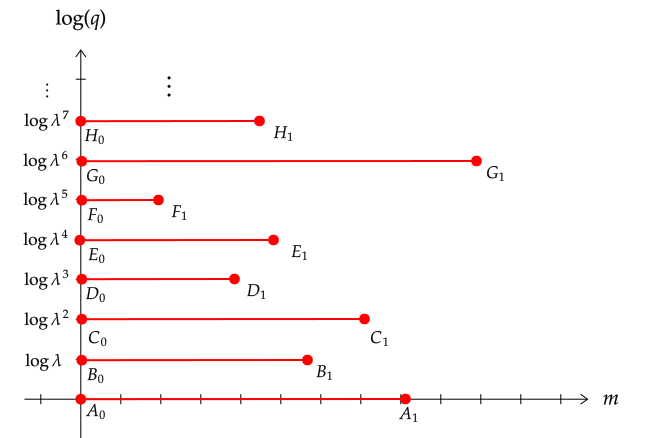
\includegraphics[scale=0.5]{figures/tikz/individual_product_line_dynamics.png}
	

\tikzset{every picture/.style={line width=0.75pt}} %set default line width to 0.75pt        

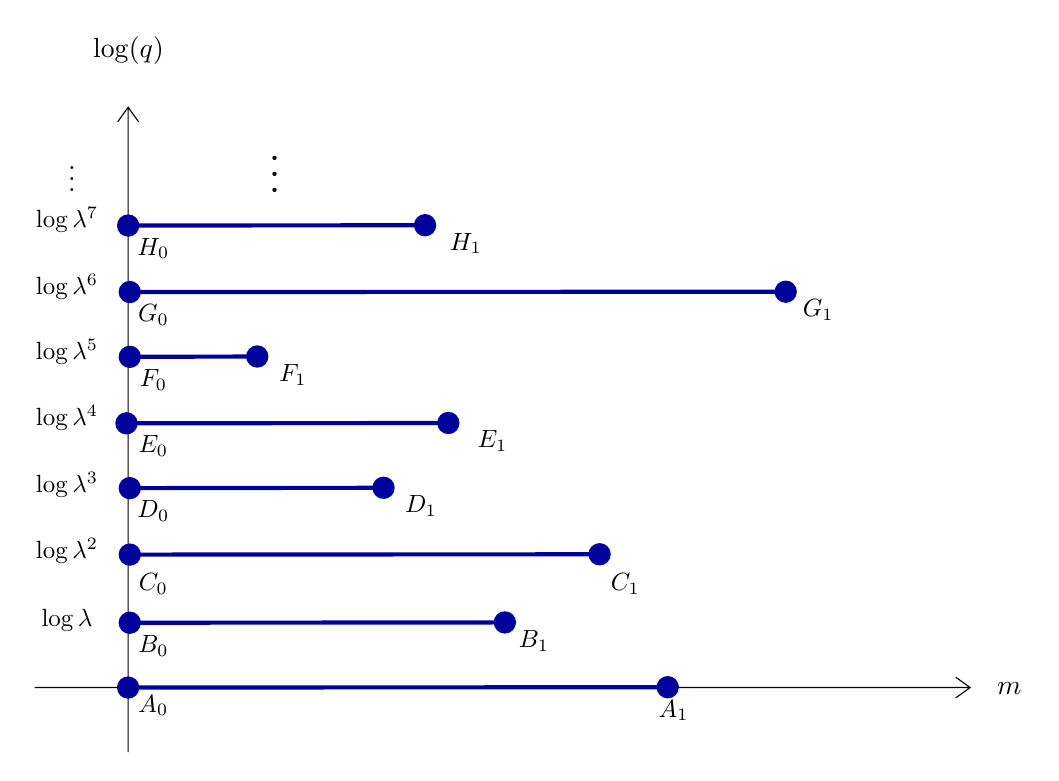
\begin{tikzpicture}[x=0.75pt,y=0.75pt,yscale=-1,xscale=1]
%uncomment if require: \path (0,436); %set diagram left start at 0, and has height of 436

%Shape: Axis 2D [id:dp5962309555056176] 
\draw  (23.9,406.93) -- (474.68,406.93)(68.98,127.34) -- (68.98,438) (467.68,401.93) -- (474.68,406.93) -- (467.68,411.93) (63.98,134.34) -- (68.98,127.34) -- (73.98,134.34)  ;
%Straight Lines [id:da5785444046568369] 
\draw [color={rgb, 255:red, 0; green, 0; blue, 155 }  ,draw opacity=1 ][line width=1.5]    (68.98,406.93) -- (328.96,406.77) ;
\draw [shift={(328.96,406.77)}, rotate = 359.96] [color={rgb, 255:red, 0; green, 0; blue, 155 }  ,draw opacity=1 ][fill={rgb, 255:red, 0; green, 0; blue, 155 }  ,fill opacity=1 ][line width=1.5]      (0, 0) circle [x radius= 4.36, y radius= 4.36]   ;
\draw [shift={(68.98,406.93)}, rotate = 359.96] [color={rgb, 255:red, 0; green, 0; blue, 155 }  ,draw opacity=1 ][fill={rgb, 255:red, 0; green, 0; blue, 155 }  ,fill opacity=1 ][line width=1.5]      (0, 0) circle [x radius= 4.36, y radius= 4.36]   ;
%Straight Lines [id:da8891623197358631] 
\draw [color={rgb, 255:red, 0; green, 0; blue, 155 }  ,draw opacity=1 ][line width=1.5]    (69.78,375.71) -- (250.49,375.55) ;
\draw [shift={(250.49,375.55)}, rotate = 359.95] [color={rgb, 255:red, 0; green, 0; blue, 155 }  ,draw opacity=1 ][fill={rgb, 255:red, 0; green, 0; blue, 155 }  ,fill opacity=1 ][line width=1.5]      (0, 0) circle [x radius= 4.36, y radius= 4.36]   ;
\draw [shift={(69.78,375.71)}, rotate = 359.95] [color={rgb, 255:red, 0; green, 0; blue, 155 }  ,draw opacity=1 ][fill={rgb, 255:red, 0; green, 0; blue, 155 }  ,fill opacity=1 ][line width=1.5]      (0, 0) circle [x radius= 4.36, y radius= 4.36]   ;
%Straight Lines [id:da62109240629908] 
\draw [color={rgb, 255:red, 0; green, 0; blue, 155 }  ,draw opacity=1 ][line width=1.5]    (69.78,342.88) -- (260.1,342.75) -- (296.13,342.72) ;
\draw [shift={(296.13,342.72)}, rotate = 359.96] [color={rgb, 255:red, 0; green, 0; blue, 155 }  ,draw opacity=1 ][fill={rgb, 255:red, 0; green, 0; blue, 155 }  ,fill opacity=1 ][line width=1.5]      (0, 0) circle [x radius= 4.36, y radius= 4.36]   ;
\draw [shift={(69.78,342.88)}, rotate = 359.96] [color={rgb, 255:red, 0; green, 0; blue, 155 }  ,draw opacity=1 ][fill={rgb, 255:red, 0; green, 0; blue, 155 }  ,fill opacity=1 ][line width=1.5]      (0, 0) circle [x radius= 4.36, y radius= 4.36]   ;
%Straight Lines [id:da3991972176156211] 
\draw [color={rgb, 255:red, 0; green, 0; blue, 155 }  ,draw opacity=1 ][line width=1.5]    (68.18,279.63) -- (223.27,279.47) ;
\draw [shift={(223.27,279.47)}, rotate = 359.94] [color={rgb, 255:red, 0; green, 0; blue, 155 }  ,draw opacity=1 ][fill={rgb, 255:red, 0; green, 0; blue, 155 }  ,fill opacity=1 ][line width=1.5]      (0, 0) circle [x radius= 4.36, y radius= 4.36]   ;
\draw [shift={(68.18,279.63)}, rotate = 359.94] [color={rgb, 255:red, 0; green, 0; blue, 155 }  ,draw opacity=1 ][fill={rgb, 255:red, 0; green, 0; blue, 155 }  ,fill opacity=1 ][line width=1.5]      (0, 0) circle [x radius= 4.36, y radius= 4.36]   ;
%Straight Lines [id:da08688218265034209] 
\draw [color={rgb, 255:red, 0; green, 0; blue, 155 }  ,draw opacity=1 ][line width=1.5]    (69.78,310.85) -- (192.04,310.69) ;
\draw [shift={(192.04,310.69)}, rotate = 359.92] [color={rgb, 255:red, 0; green, 0; blue, 155 }  ,draw opacity=1 ][fill={rgb, 255:red, 0; green, 0; blue, 155 }  ,fill opacity=1 ][line width=1.5]      (0, 0) circle [x radius= 4.36, y radius= 4.36]   ;
\draw [shift={(69.78,310.85)}, rotate = 359.92] [color={rgb, 255:red, 0; green, 0; blue, 155 }  ,draw opacity=1 ][fill={rgb, 255:red, 0; green, 0; blue, 155 }  ,fill opacity=1 ][line width=1.5]      (0, 0) circle [x radius= 4.36, y radius= 4.36]   ;
%Straight Lines [id:da027938631411597137] 
\draw [color={rgb, 255:red, 0; green, 0; blue, 155 }  ,draw opacity=1 ][line width=1.5]    (69.78,247.6) -- (131.19,247.44) ;
\draw [shift={(131.19,247.44)}, rotate = 359.85] [color={rgb, 255:red, 0; green, 0; blue, 155 }  ,draw opacity=1 ][fill={rgb, 255:red, 0; green, 0; blue, 155 }  ,fill opacity=1 ][line width=1.5]      (0, 0) circle [x radius= 4.36, y radius= 4.36]   ;
\draw [shift={(69.78,247.6)}, rotate = 359.85] [color={rgb, 255:red, 0; green, 0; blue, 155 }  ,draw opacity=1 ][fill={rgb, 255:red, 0; green, 0; blue, 155 }  ,fill opacity=1 ][line width=1.5]      (0, 0) circle [x radius= 4.36, y radius= 4.36]   ;
%Straight Lines [id:da3281189416601338] 
\draw [color={rgb, 255:red, 0; green, 0; blue, 155 }  ,draw opacity=1 ][line width=1.5]    (69.78,216.38) -- (385.8,216.22) ;
\draw [shift={(385.8,216.22)}, rotate = 359.97] [color={rgb, 255:red, 0; green, 0; blue, 155 }  ,draw opacity=1 ][fill={rgb, 255:red, 0; green, 0; blue, 155 }  ,fill opacity=1 ][line width=1.5]      (0, 0) circle [x radius= 4.36, y radius= 4.36]   ;
\draw [shift={(69.78,216.38)}, rotate = 359.97] [color={rgb, 255:red, 0; green, 0; blue, 155 }  ,draw opacity=1 ][fill={rgb, 255:red, 0; green, 0; blue, 155 }  ,fill opacity=1 ][line width=1.5]      (0, 0) circle [x radius= 4.36, y radius= 4.36]   ;
%Straight Lines [id:da5404789458766659] 
\draw [color={rgb, 255:red, 0; green, 0; blue, 155 }  ,draw opacity=1 ][line width=1.5]    (68.98,184.35) -- (212.06,184.19) ;
\draw [shift={(212.06,184.19)}, rotate = 359.94] [color={rgb, 255:red, 0; green, 0; blue, 155 }  ,draw opacity=1 ][fill={rgb, 255:red, 0; green, 0; blue, 155 }  ,fill opacity=1 ][line width=1.5]      (0, 0) circle [x radius= 4.36, y radius= 4.36]   ;
\draw [shift={(68.98,184.35)}, rotate = 359.94] [color={rgb, 255:red, 0; green, 0; blue, 155 }  ,draw opacity=1 ][fill={rgb, 255:red, 0; green, 0; blue, 155 }  ,fill opacity=1 ][line width=1.5]      (0, 0) circle [x radius= 4.36, y radius= 4.36]   ;

% Text Node
\draw (39.52,374.75) node [scale=0.9]  {$\log \lambda $};
% Text Node
\draw (69.14,100.12) node [scale=1]  {$\log( q)$};
% Text Node
\draw (493.49,407.37) node [scale=1]  {$m$};
% Text Node
\draw (39.52,341.12) node [scale=0.9]  {$\log \lambda ^{2}$};
% Text Node
\draw (39.52,309.09) node [scale=0.9]  {$\log \lambda ^{3}$};
% Text Node
\draw (39.52,277.07) node [scale=0.9]  {$\log \lambda ^{4}$};
% Text Node
\draw (39.52,245.04) node [scale=0.9]  {$\log \lambda ^{5}$};
% Text Node
\draw (39.52,213.81) node [scale=0.9]  {$\log \lambda ^{6}$};
% Text Node
\draw (39.52,181.79) node [scale=0.9]  {$\log \lambda ^{7}$};
% Text Node
\draw (81.15,415.58) node [scale=0.9]  {$A_{0}$};
% Text Node
\draw (331.76,417.98) node [scale=0.9]  {$A_{1}$};
% Text Node
\draw (81.15,386.76) node [scale=0.9]  {$B_{0}$};
% Text Node
\draw (264.5,384.36) node [scale=0.9]  {$B_{1}$};
% Text Node
\draw (81.15,357.13) node [scale=0.9]  {$C_{0}$};
% Text Node
\draw (308.54,357.13) node [scale=0.9]  {$C_{1}$};
% Text Node
\draw (41.92,157.77) node   {$\vdots $};
% Text Node
\draw (81.15,290.68) node [scale=0.9]  {$E_{0}$};
% Text Node
\draw (244.49,288.28) node [scale=0.9]  {$E_{1}$};
% Text Node
\draw (81.15,321.9) node [scale=0.9]  {$D_{0}$};
% Text Node
\draw (210.06,319.5) node [scale=0.9]  {$D_{1}$};
% Text Node
\draw (81.15,258.65) node [scale=0.9]  {$F_{0}$};
% Text Node
\draw (148.41,256.25) node [scale=0.9]  {$F_{1}$};
% Text Node
\draw (81.15,227.42) node [scale=0.9]  {$G_{0}$};
% Text Node
\draw (401.42,225.02) node [scale=0.9]  {$G_{1}$};
% Text Node
\draw (81.15,195.4) node [scale=0.9]  {$H_{0}$};
% Text Node
\draw (231.68,193) node [scale=0.9]  {$H_{1}$};
% Text Node
\draw (139.6,153.76) node [scale=1.44]  {$\vdots $};


\end{tikzpicture}

	\caption{This figure illustrates the dynamics of an individual product line in the equilibrium of the model. All product lines start at point $A_0$. A typical path is given by the red lines, moving left to right to $A_1$ then jumping to $B_0$ before continuing to drift to $B_1$, jump to $C_0$, and so on.}
	\label{individual_product_line_dynamics}
\end{figure}





\subsection{Equilibrium}

I will solve for an equilibrium of the model which is a balanced growth path. In such an equilibrium, output, consumption and average quality in the economy grow at a constant and equal exponential rate and 

\subsubsection{Basics}

Household risk-neutrality implies $r_t \equiv \rho$.

\subsubsection{Static optimization}

\paragraph{Quality gaps and limit pricing} Let $\bar{q}_j(t)$ denote the highest quality level of good $j$ available in the economy at time $t$. Typically, there would be limit pricing, and the markup charged by the technology leader in line $j$ would depend on his gap relative to the next laggard, e.g. \cite{baslandze_spinout_2019} or \cite{aghion_competition_2005}, only equating to the monopolistic competition markup for large enough gaps. In my model, for the sake of simplicity, I abstract from limit pricing, using an assumption from \cite{akcigit_growth_2018}. At each time $t$, intermediate goods firms play a two-stage Bertrand competition game. In the first stage, participants bear a cost of $\varepsilon > 0$ units of the final good in exchange for a right to compete in the product market. In the second stage, they engage in Bertrand competition. Limit pricing in the second stage Bertrand game implies that all producers not on the frontier will earn zero profits; therefore, they do not pay the entry cost. In equilibrium, the leader can charge the optimal monopolistic competition markup, regardless of $\lambda$. This reduces the state space of the incumbents' optimization problem by one dimension, since the technological gap no longer needs to be tracked to determine optimal pricing.

The model gains significant tractability from the fact that static production decisions are entirely separable from dynamic R\&D decisions. Below I solve the equilibrium fo the static side of the model, given an allocation to R\&D labor $L_{RD}$. 

Final goods producer optimization implies the following inverse demand function for intermediate goods, 
\begin{align*}
p_j &= L_F^{\beta} q_j^{\beta} k_j^{-\beta}	
\end{align*}

Profit maximization for intermediate goods producers yields
\begin{align}
\pi(q_j) = \max_{k_j \ge 0} \Big\{ L_F^{\beta} q_j^{\beta} k_j^{1-\beta} - \frac{\overline{w}}{Q} \Big\} \label{incumbent_profit}
\end{align}

where $\overline{w}$ is the equilibrium final goods / intermediate goods wage.
This yields optimal pricing, labor demand and production of intermediate goods,
\begin{align}
k_j &= \Big[ \frac{(1-\beta) Q}{\overline{w}} L_F q_j  \Big] \label{optimal_k}\\
l_j &= k_j / Q \label{optimal_l}\\
p_j &= \frac{\overline{w}}{(1-\beta) Q} \label{optimal_p}\\
C(\beta) &= \Big(\frac{\beta}{1-\beta} (1-\beta)^{\frac{1-\beta}{\beta}} \Big)^{\beta} \label{def_cbeta}
\end{align}

Substituting (\ref{optimal_k}) into the first-order condition for final goods firm optimal labor demand yields a closed form expression for the equilibrium wage $\overline{w}$:
\begin{align}
\overline{w} &= C(\beta) Q \label{wbar}
\end{align}

Substituting (\ref{optimal_p}) and (\ref{wbar}) into (\ref{incumbent_profit}) and optimizing
\begin{align}
\pi_j &= \beta L_F q_j \label{profits_eq}
\end{align}

Substituting (\ref{optimal_k}) into (\ref{optimal_l}) and integrating $L_I = \int_0^1 l_j dj$ yields aggregate labor allocated to intermediate goods production,
\begin{align}
L_I &= \frac{1-\beta}{C(\beta)}L_F \label{intermediate_goods_labor}
\end{align}

Plugging (\ref{optimal_k}) into (\ref{final_goods_production}) yields
\begin{align}
Y = \frac{(1-\beta)^{1-2\beta}}{\beta^{1-\beta}} Q L_F
\end{align}

and substituting (\ref{intermediate_goods_labor}) into the labor resource constraint (\ref{labor_resource_constraint}) yields
\begin{align}
L_F &= \frac{1 - L_{RD}}{1 + \frac{1-\beta}{C(\beta)}}
\end{align}

The value of $L_{RD}$ is determined by the R\&D side of the model, described below.

\subsubsection{Dynamic optimization}

The state variable of a product $j$ is $(q,m,t)$, where $q$ is the currently available highest quality, $m$ is the mass of spinouts capable of attempting entry and $t$ allows dependence on time-varying rates of creative destruction or economy-wide average quality $Q = \int_{q,m} q  \cdot d\mu(q,m,t)$. Let $W(q,m,t)$ denote value per spinout idea in state $(q,m)$ at time $t$. 

The equilibrium wage paid to R\&D workers not bound by non-competes will depend on the individual state of the product, as this affects the value of the spinouts ideas generated by the R\&D worker. Let $w^{NCA}(q,m,t),w(q,m,t)$ denote the equilibrium wages required by R\&D employees bound (not bound) by an NCA.

\paragraph{Households}

Individuals are risk neutral and can borrow and lend instantaneous risk-free bonds. This implies that their objective is to maximize the present discounted value of their wages and profits from founding firms. Because founding and owning a firm does not require labor, entrepreneurship decisions are completely separate from labor supply decisions. Labor supply is allocated in order to maximize the value of the labor endowment. Denote this value by $U_{labor}$. It satisfies the HJB equation
\begin{align}
\rho U_{labor} &= \max_{l_{q,m}(\cdot),l_I,l_F} \bar{w}(t) (l_I + l_F) \nonumber\\
&+ \int_{q,m} l_{RD} (q,m) \Bigg(x(q,m,t) \hat{w}^{NCA}(q,m,t) + \Big(1-x(q,m,t) \Big)\hat{w}(q,m,t))  \Bigg) d\mu(q,m,t) \nonumber  \\
\textrm{subject to: }  & l_{RD}(\cdot) \ge 0, l_I \ge 0, l_F \ge 0  \nonumber \\
& l_I + l_F + \int_{q,m} l_{RD}(q,m) d\mu(q,m,t) \le 1 
\end{align}

where $x(q,m,t)$ is equal to 1 if and only if product lines in state $(q,m,t)$ require non-competes, $l_{RD}(q,m)$ is the average labor supplied by the individual to products in state $(q,m)$,  $\bar{w}(t)$ is the production wage and $\hat{w}^{NCA}(q,m,t),\hat{w}(q,m,t)$ are the effective R\&D wages from the perspective of the employee bound / not-bound by a non-compete, respectively, taking into account the profits from future spinouts: 
\begin{align}
\hat{w}(q,m,t) &=  w(q,m,t) + \nu \Big( \overbrace{\theta \frac{Q_t}{q} W(\lambda q,0,t)}^{\textrm{WSOs}} + \overbrace{(1-\theta) \mathcal{W}(t)}^{\textrm{Non-WSOs}} \Big) \label{worker_effective_wage}\\
\hat{w}^{NCA}(q,m,t) &= w^{NCA}(q,m,t) + \nu \underbrace{(1-\theta) \mathcal{W}(t)}_{\textrm{Only Non-WSOs}} \label{worker_effective_wage_NCA}\\ 
\mathcal{W}(t) &= \int_{q,m} W(\lambda q,m,t) d\mu(q,m,t)
\end{align}

In equilibrium, the worker is indifferent between all forms of employment. This means that whenever $x(q,m,t) = 1$, 
\begin{align}
\hat{w}^{NCA}(q,m,t) &= \bar{w}(t) \label{wage_rd_NCA}
\end{align}

and when $x(q,m,t) = 0$, 
\begin{align}
\hat{w}(q,m,t) &= \bar{w}(t) \label{wage_rd}
\end{align}


\paragraph{Incumbents}

Let $\pi(q,m,t) = \pi q$ denote flow profits from sales of the intermediate good and let $\tau(q,m,t) = \tau_E(q,m,t) + \tau_S(q,m,t)$ denote the arrival rate of creative destruction by entrants and spinouts. 

The incumbent value function satisfies the HJB equation
\begin{align}
	\big(\rho + \tau^E(q,m,t)& \big)V(q,m,t) = \pi q + \bar{\sigma} V_m + V_t  \nonumber \\
	                           &+ \max_{x \in \{0,1\}, z \ge 0} \Bigg\{ z \Big( z^{-\psi_I} \chi_I \big( V(\lambda q, 0, t) - V(q,m,t) \big)  \nonumber \\
	                           &- x w^{NCA}(q,m,t) - (1-x) \big(w(q,m,t) - \theta \nu V_m \big)\Big)    \Bigg\}
\end{align}

Define the incumbent's effective cost of R\&D both with and without an NCA,
\begin{align}
\tilde{w}^{NCA}(q,m,t) &= w^{NCA}(q,m,t)  \label{incumbent_effective_wage_NCA} \\
\tilde{w}(q,m,t) &= w(q,m,t) - \theta \nu V_m(q,m,t)  \label{incumbent_effective_wage}
\end{align}

That is, the effective cost of R\&D is the nominal cost of R\&D plus the reduction in firm value from the resulting marginal increase in the stock of spinouts attempting entry, $m$. This is because higher $m$ implies a higher hazard rate of losing the monopoly position. It follows from the HJB that the incumbent uses a non-compete (chooses $x = 1$) whenever it means his effective cost of R\&D is lower: $\tilde{w} > \tilde{w}^{NCA}$. 

A higher wage is required to attract labor when a non-compete is imposed, since it eliminates the expected value of the employee's future WSOs. The gap in wages required to attract labor is equal to the expected discounted present value of WSO formation to the worker. Using (\ref{worker_effective_wage}), (\ref{incumbent_effective_wage_NCA}), and (\ref{incumbent_effective_wage}), and the indifference condition (\ref{wage_rd}), it follows that
\begin{align}
\tilde{w}^{NCA} &= \tilde{w}(m) + \underbrace{\theta \nu V'(m)}_{\textrm{Expected cost to incumbent}} + \overbrace{\nu \theta W(m) }^{\textrm{Expected value to worker}}
\end{align} 

That is, the incumbent uses a non-compete whenever the ex-ante bilateral value of knowledge spillovers from the incumbent to the R\&D employee is positive. Equilibrium thus achieves the bilaterally optimal contract in the available contracting space. Negative social consequences of non-competes in this model therefore arise from externalities and general equilibrium effects rather than direct harm to those bound by them.\footnote{This is also the case in the models developed in \cite{baslandze_spinout_2019} and \cite{shi_restrictions_2018}. However, there is empirical evidence that non-compete contracts can be damaging to workers themselves. Essentially, in some cases a non-compete can be used as a way to extract more rent from the worker after a job has already been accepted. It appears that additional compensation is received under non-competition agreements only in states in which such practices are prevented by "Consideration" requirements for new non-compete contracts. See the discussion in \cite{starr_consider_2018}.}

Finally, optimal R\&D policy is determined by the first-order condition
\begin{align}
	z^*(q,m,t) &= \Bigg( \frac{x^*(q,m,t) \tilde{w}^{NCA}(q,m,t) + (1-x^*(q,m,t))\tilde{w}(q,m,t)}{\chi_I(1-\psi_I) \Big(V(\lambda q, 0, t) - V(q,m,t) \Big)}\Bigg)^{-1/\psi_I}
\end{align}

\paragraph{Spinouts}

The value of a spinout idea $W(q,m,t)$ satisfies the HJB
\begin{align}
(\rho  + \tau_E + \tau_S& + \tau_I)W(q,m,t) = W_t(q,m,t) + \bar{\sigma}W_m(q,m,t) \nonumber \\
+& \max_{0 \le z \le 1} \Big\{ \underbrace{\chi_S z (z_E + z_S)^{-\psi_{SE}} (1-\kappa) V(\lambda q,0,t)}_{\textrm{Flow value of potential innovation}} - \underbrace{\Big(\frac{q}{Q_t}\Big) z w(q,m,t)}_{\textrm{R\&D cost}} \Big\} \label{HJB_S}
\end{align}

There are three important differences relative to the incumbent's problem. First, because each spinout is infinitesimal, individual spinouts in line $j$ have no effect on the overall creative destruction rate in line $j$. Second, because employment at spinouts does not generate further spinout ideas for employees, spinouts pay the production wage for R\&D employees. As mentioned before, this can be relaxed, but I have no data on R\&D by spinouts with which to discipline the necessary parameters.\footnote{If this were relaxed, because spinouts are infinitesimal, their effective wage paid would equal the nominal wage, because they have no individual effect on the dynamics of the state variable $m_j$.} 

Finally a cost $\kappa V(\lambda q, 0, t)$ must be paid upon entry. This directly reduces the value of spinout formation. However, because (1) spinout ideas are generated as a by-product of R\&D decisions made by the firm, and (2) $\chi_S > \chi_E$ so that spinout ideas are not marginal (ordinary entrants act as a "buffer") and (3) spinouts are individually CRS with a capacity constraint so always operate at the same capacity, the rate of spinout formation is relatively unaffected by an increase in $\kappa$\footnote{It begins to be affected when spinouts are marginal entrants, but this is unlikely in equilibrium since it requires many spinout ideas to have leaked already; typically an innovation occurs before this happens, rendering previous spinouts obsolete and resetting $m$ to zero.}. By the logic above, then, a high value of the parameter $\kappa$ makes NCAs bilaterally optimal. Note also that, for this conclusion, it is not essential whether the cost $\kappa$ is thought of as a payment to factors of production or a transfer to financiers which does not consume societal resources. This distinction is, however, important for the calculation of total welfare. In any case, in the calibrations I explore in this paper, it will turn out that the welfare implications are not driven by the direct cost of new firm formation, but rather by the effect of $\kappa$ on R\&D expenditures of incumbents, spinouts and ordinary entrants. 

\paragraph{Equilibrium entry behavior}

Free entry by ordinary entrants imposes the following condition on $z_E(q,m,t)$, 
\begin{align}
\chi_E \big( z_E(q,m,t) + z_S(q,m,t) \big)^{-\psi_{SE}} \Big(\frac{q}{Q_t}\Big)^{-1}  (1-\kappa) V(\lambda q,0,t)  &= \bar{w}(t)\label{free_entry_entrants}
\end{align}
with equality if $z_E(q,m,t) > 0$. 

Provided that $\chi_S > \chi_E$, spinouts price ordinary entrants out of the innovation race as $m$ increases. During this process, free entry of ordinary entrants implies that $z_S(q,m,t) + z_E(q,m,t)$ remains constant. Once $z_E(q,m,t) = 0$, spinouts continue to enter until $m$ reaches the free entry mass $M(q,t) > 0$ defined by
\begin{align}
\chi_S  M(q,t)^{-\psi_{SE}}\Big(\frac{q}{Q_t}\Big)^{-1} (1-\kappa) V(\lambda q,0,t)  &= \overline{w}(t) \label{free_entry_spinouts}
\end{align}

That is, for $m \ge M(q,t)$ have $z_S(q,m,t) = M(q,t)$ and for $m < M(q,t)$ have $z_S(m,q,t) = m$. 


\subsubsection{Linear scaling in $q$}

I guess and verify that $V(q,m,t) = q V(m)$ and $W(q,m,t) = qW(m)$ for some functions $V(m)$ and $W(m)$, abusing notation. Similarly, I conjecture that $x,z_I,z_E,zS,\tau_E,\tau_S$ are functions of $m$ exclusively, and that $L_F,L_I,L_{RD}$ are constant, which by (\ref{profits_eq}) implies that $\pi(q,m,t) = \pi q$. Then $\bar{w}(t) = Q_t \bar{w}$ and (\ref{wage_rd_NCA}), (\ref{wage_rd}) imply that $w(q,m,t) = Q_t w(m),w^{NCA}(q,m,t) = Q_tw^{NCA}(m)$ and similarly for $\hat{w}(q,m,t),\hat{w}^{NCA}(q,m,t),\tilde{w}(q,m,t),$ and $\tilde{w}^{NCA}(q,m,t)$. 

To verify the guess, a factor $q$ drops out of (\ref{HJB_I}) and (\ref{HJB_S}), yielding
\begin{align}
(r + \tau_E(m) + &\tau_S(m)) V(m) = \pi + \bar{\sigma}V'(m) \nonumber \\
&+ \max_{z \ge 0, x \in \{0,1\}} \Big\{  \chi_I z \phi_I(z) \Big[\lambda V(0) - V(m) \Big] - z \Big(x \tilde{w}^{NCA}(m) + (1-x) \tilde{w}(m) \Big) \Big\} \label{BGP_HJB_I}
\end{align} 
and 
\begin{align}
(r + \tau_E(m) + &\tau_S(m) + \tau_I(m))W(m) = \sigma(m) W'(m) \nonumber \\
&+ \max_{0 \le z \le \xi} \Big\{  \chi_S z (z_E(m) + z_S(m))^{-\psi_{SE}} (1-\kappa) \lambda V(0) - z \bar{w} \Big\} \label{BGP_HJB_S} 
\end{align}

where
\begin{align}
\sigma(m) &= \nu \theta z_I(m) + \bar{\sigma} 
\end{align}

Finally, optimal policies are functions of only $m$ as well, 
\begin{align}
x^*(m) &= \textbf{1}_{\tilde{w}(m) > \tilde{w}^{NCA}(m)} \big(m\big) \\
z_I^*(m) &= \Bigg( \frac{x^*(m) \tilde{w}^{NCA}(m) + (1-x^*(m)) \tilde{w}(m)}{\chi_I (1-\psi) \Big(\lambda V(0) - V(m) \Big)} \Bigg)^{-1/\psi_I} \\
z_E^*(m) &= \max \Bigg\{0, \Big(\frac{\overline{w}}{\chi_E (1-\kappa) \lambda V(0)} \Big)^{-1 / \psi_{SE}} - z_S^*(m)\Bigg\} \\
z_S^*(m) &= \min(m,M^*) \\
M^* &= \Big(\frac{\overline{w}}{\chi_S (1-\kappa) \lambda V(0)} \Big)^{-1 / \psi_{SE}}
\end{align}

\subsubsection{Balanced growth path}\label{bgp}

\paragraph{Aggregate distributions} 

On the balanced growth path, $Q_t = \int_{q,m} d\mu(q,m,t)$ grows at a constant rate $g$. There is no stationary distribution in $(q,m)$-space due to this growth. In addition, there is no stationary distribution in $(q/Q_t,m)$-space due to growth rates constant in $q/Q$ and no low exit barrier, which creates a "fanning out" of the distribution over time. Instead, there is a stationary distribution in $m$-space, with density $\mu(m)$, together with a function $\gamma(m) = \mathbb{E}_t[q/Q_t|m]$. The density $\mu(m)$ satisfies Kolmogorov Forward Equation
\begin{align}
0 = - \frac{d}{dm} \Big( \sigma(m) \mu(m) \Big) - \tau(m) \mu(m)  \label{KF_equation}
\end{align}
where
\begin{align}
\tau(m) &= \tau_I(m) + \tau_S(m) + \tau_E(m) 
\end{align}

This ODE has solutions of the form
\begin{align}
\mu(m) &= C_\mu e^{-\int_0^m \frac{\sigma'(m') + \tau(m')}{\sigma(m')}} dm' \label{KF_solution_1}
\end{align}

Because $\mu(m)$ is a probability density function, $C_\mu$ is determined by
\begin{align}
1 = \int_0^{\infty} \mu(m) dm \label{KF_solution_2}
\end{align}

To compute $\gamma(m)$, define $s(m)$ as the equilibrium (deterministic) amount of time to reach state $m$ from state $0$, conditional on no intervening innovations), 
\begin{align}
s(m) &= \int_0^m \frac{1}{\sigma(m')} dm'
\end{align}

Define $\tilde{\gamma}(s') = \gamma(s^{-1}(s'))$. Absent any innovation, $q/Q_t$ decreases at rate $g$. Therefore, $\gamma(s)$ decays at rate $g$, 
\begin{align}
\tilde{\gamma}(s) &= C_{\gamma} e^{-gs}
\end{align}

Recover $\gamma(m)$ using 
\begin{align}
\gamma(m) &= \tilde{\gamma}(s(m))
\end{align}

Finally, $C_{\gamma}$ is determined by \footnote{It is possible to also derive the condition $C_{\gamma} = \lambda \int_0^{\infty} \gamma(m) \tau(m) \mu(m) dm$. This equation can be shown to be redundant.}
\begin{align}
\int_0^{\infty} \gamma(m) \mu(m) dm = 1
\end{align}

\paragraph{Aggregate growth and R\&D labor demand}

Given aggregate distributions $\mu(m),\gamma(m)$ and product-level innovation rates $\tau(m) = \tau_I(m) + \tau_S(m) + \tau_E(m)$, the growth rate of TFP is given by
\begin{align}
g &= (\lambda -1) \int_0^{\infty} \tau(m) \gamma(m) \mu(m) dm 
\end{align}

The growth equation aggregates across products in $m$-space using the stationary density $\mu(m)$. For each $m$, the contribution to growth is the product of the rate of innovation $\tau(m)$, the average relative quality $\gamma(m)$, and $(\lambda -1)$, the proportional improvement in quality per innovation.

R\&D labor demand is given by 
\begin{align*}
L_{RD} &= \int_0^{\infty} \big (z_I(m) + z_S(m) + z_E(m)\big)\gamma(m)\mu(m) dm
\end{align*}

\subsubsection{Solution algorithm}\label{solution_algorithm}

The HJBs given above cannot be solved in closed form. I solve them using a variant of the numerical method described in using method in \cite{achdou_income_2017}. I can then solve the model numerically using the following algorithm.

\begin{enumerate}
	\item Guess $\{g, L_{RD}, w(m), w^{NC}, M, \bar{\sigma} \}$
	\begin{enumerate}
		\item Static equilibrium conditions $\Rightarrow L_I,L_F,\pi$
		\begin{enumerate}
			\item Free entry, etc. $\Rightarrow z_S(m), z_E(m)$
			\item Incumbent HJB $\Rightarrow  V(m),z_I(m)$ 
			\item Update $M$ and check for convergence
		\end{enumerate}
		\item Spinout HJB $\Rightarrow$ $W(m)$
		\item Aggregation $\Rightarrow$ $\mu(m),\gamma(m),g,L_{RD},\bar{\sigma},\mathcal{W}$
		\item Worker indifference $\Rightarrow$ $w(m),w^{NC}$
		\item Check convergence of of $\{g, L_{RD}, w(m), w^{NC}, M, \bar{\sigma} \}$
	\end{enumerate}
\end{enumerate}


\subsection{Efficiency}

The social planner problem now involves controlling the infinite dimensional aggregate state variable $\mu(\cdot), \gamma(\cdot)$ as well as infinite dimensional individual policy functions $z_S(\cdot),z_E(\cdot),z_I(\cdot)$ to maximize welfare, given market clearing and the steady state KF and $\gamma$ equations. I plan to adapt the methods in \cite{nuno_social_2018} to compute the social planner's allocation numerically. Given risk-neutrality, expected utility for a household born in this economy is equal to the expected discounted present value of consumption in the economy at time $t = 0$ with $Q_0 = 1$. 


\section{Empirics}\label{Empirics}

The purpose this section is (1) to provide some empirical motivation for the model used for counterfactual analysis, and (2) to provide some estimates which can be used to discipline the parametrization of the same model. 

\subsection{Data}

The empirical component uses microeconomic data from three sources: Venture Source, Compustat, and the NBER-USPTO patent database.

\paragraph{Venture Source}

Venture Source is a proprietary dataset containing information on venture capital-funded startups, their investors and their key employees. I use a subsample of the data for US-based startups founded between 1986 and 2008. The data cover 23,434 startups, 89,382 financing rounds, and 297,119 employee-firm pairs. For each startup, the data has the founding date of the firm and the join dates and, importantly, a chronological list of the previous employers of all founders, C-level employees, and some board members. In addition, for each financing round, the data contain information on valuation, amount raised, and status of the business at the time of the round (e.g., product development, generating revenue, profitable). The dataset is described in detail in \cite{kaplan_how_2002} and \cite{kaplan_venture_2016}. 

\paragraph{Compustat}

The second dataset I employ is Compustat. I consider the subsample of all firms headquartered in the United States in operation at any point between 1986 and 2006, consisting of 21,110 firms. The Compustat data has information on R\&D expenditures at the firm-year level as well as time-varying firm controls.

\paragraph{NBER-USPTO Patent data}

The NBER-USPTO database contains comprehensive information on all patents granted in the United States from 1976 to 2006, and is linked to Compustat. I consider the subsample of patents assigned to US firms, consisting of 1,457,136 patents. 

\subsubsection{Construction of dataset}

I begin by linking firms in Compustat to their employee spinouts in Venture Source. I define a startup $s$ as a spinout of a firm $f$ in Compustat if its CTO, CEO, Chairman, President or Founder (1) most recently worked at firm $f$ prior to joining firm $s$ and (2) joined firm $s$ in its first three years.

Performing this match requires linking observations by the string describing the firm name, which poses a challenge because firms can go by different names. Minor differences in conventions (e.g. "Corp" vs "Corp.") can be handled by using regular expressions. Parent firms which are subsidiaries of firms in Compustat can be linked using Compustat data on firm subsidiaries. Sometimes subsidiaries are not listed in Compustat or firms go by completely different names, e.g., "Advanced Micro Devices" and "AMD."  In these cases, I use the merchant-mapper tool from Alternative Data Group, an application which is able to link an unstructured string to a corresponding firm. This link also provides a stock exchange ticker symbol, which I use to match the firm to Compustat.\footnote{The tool was designed for use by hedge funds, for linking e.g. credit card transaction data to firms. Alternative Data Group is itself an employee spinout of 1010 data, another data processing and analysis firm.} Using this approach, I identify 8,420 spinouts founded between 1986 and 2008, linked to 3,410 parent firms in Compustat. On a founder-weighted basis, I identify 4,595 spinouts.

Because my analysis focuses on creative destruction by employee spinouts, it is important to quantify the extent to which spinout firms directly compete with their parent firms. While the Venture Source data do not include NAICS codes, they do provide detailed industry information at a similar level of aggregation. The scheme is roughly consistent, as most Venture Source industry categories coincide with 4-digit NAICS codes. Therefore, I proceed by manually constructing a cross-walk.

Finally, I link the resulting dataset to patent data using the NBER-USPTO patent dataset. This is straightforward because I am only interested in matching patents to parent firms in Compustat, which have previously been linked to the NBER-USPTO data.

\subsection{Measuring spinout formation}

I construct three measures of employee spinout formation. \textbf{Founder counts}, consists of the number of founders most recently employed at $f$ who join startups in years $t+1$ and $t+2$. \textbf{spinout counts} consists of a weighted count of founders previously employed at $f$ joining startups in years $t+1$ and $t+2$. The weight for a founder of startup $s$ with $N_s$ founders is $1/N_s$. The purpose of this weighting scheme is to avoid double-counting spinouts. Finally, for each spinout $s$ consider the valuation at its first funding date and discount this to the founding date using a discount rate of $5\%$, consistent with the calibration. The \textbf{spinout discounted first funding valuation (DFFV)} for firm $f$ in year $t$ is the sum of the discounted first funding valuation across spinouts formed in years $t+1,t+2$ by employees most recently employeed at $f$. 

Figure \ref{spinout_entrants_counts_unweighted} shows the count of startups founded in each year, broken down into same-NAICS 4 spinouts (WSO4 spinouts), non-WSO4 spinouts, and non-spinouts. In the typical year, 30.4\% of entering firms are spinouts and 10.3\% are WSO4 spinouts. Overall, spinouts and WSO4 spinouts make up 35.9\% and 13.1\% of the sample, respectively. These figures are broadly consistent with prior findings, albeit using other datasets and slightly different definitions of employee spinouts. For example, using US patent data, \cite{baslandze_spinout_2019} finds that 25\% of entering firms are spinouts in any industry (defined as firms with patenting employees who previously patented). Using Brazilian administrative data, \cite{muendler_employee_2012} finds that 16.9\% of entering firms are spinouts in the same CNAE 4-digit industry, when using a founder-based definition of spinouts. My lower estimate is at least partly due to my sample of parents being restricted to public firms. 

Figure \ref{spinout_entrants_counts_weighted} shows firm counts weighted to take into account the fraction of founders which were last employed at a Compustat firm. Figure \ref{spinout_entrants_foundercounts} shows counts of founders. 37\% of founders in the dataset can be traced to a Compustat firm. Previously, \cite{gompers_entrepreneurial_2005} found a figure of approximately 30-35\% using the same dataset. I am in the process of validating this match, mainly to ensure subsidiaries are not being linked to parent firms before they are acquired by them (since my AltDG algorithm only knows current parent-subsidiary relationships). Still, the results don't change much if I only consider the spinouts I have personally validated.

\begin{figure}[p]
	\centering
	\includegraphics[scale=0.8]{../figures/spinouts_entrants_counts.png}
	\caption{Results of spinout identification procedure.}
	\label{spinout_entrants_counts_unweighted}
\end{figure}


\subsection{Corporate R\&D and spinout formation}

In this section I document a relationship between parent firm R\&D and formation of spinouts by employees.

\begin{figure}[p]
	\centering
	\includegraphics[scale=0.8]{../figures/scatterPlot_RD-Spinouts-1yr-allFE.png}
	\caption{Devations of R\&D spending and spinout counts at firm-year from firm, firm age, NAICS4-year and state-year means.}
	\label{scatter_rd_spinoutcounts_d}
\end{figure}

Figures \ref{scatter_rd_spinoutcounts} and \ref{scatter_rd_spinoutcounts_d} show the firm-year level relationship between R\&D spending and spinout counts, demeaned by firm, firm age, industry-year and state-year. Figures \ref{scatter_rd_foundercounts}, \ref{scatter_rd_foundercounts_d}, \ref{scatter_rd_dffv}, and \ref{scatter_rd_dffv_d} show the same plots for founder counts and DFFV, respectively. While the data are noisy, all of the plots show a positive relationship, and it is robust to the addition of demeaning. These graphical intuitions are confirmed in the next section.

\subsubsection{Regression analysis}

In this section I consider the effect of R\&D at a firm in time $t$ on spinout formation by its employees in subsequent years. One important conceptual question must be clarified. Suppose an employee $e$ joins parent firm $f$ at time $t$, leaves at $t+k$ and forms a spinout $s$ at $t+k+1$. Is $s$ counted as a spinout when considering the effect of R\&D at $f$ at times $t' < t$? I refer to the methodology which answers "no" to this question as the \textbf{employee-centric} approach; that which answers "yes" I refer to as the \textbf{firm-centric} approach. 

Conceptually speaking, the employee-centric approach captures ideas generated by employees in the process of the firm's performing R\&D. The firm-centric approach in addition captures appropriation by employees of ideas already generated by R\&D but not yet implemented. Notice that the firm-centric approach mechanically has weakly larger spinout counts than the employee-centric approach. 

In the ideal employee-centric approach, one relates R\&D at $f$ at time $t$ to spinouts $s$ formed in $t+k$ by employees who worked at $f$ at time $t$. Absent dates of previous employment, I can only approximate this method, by assuming that a founder of a startup $s$ who joins at time $t$ worked at his previous employer since $t-k$, where $k$ could be chosen based on industry-specific, region-specific, year-specific average job tenures. The firm-centric approach, on the other hand, is implementable with my data, as it only requires knowing that the employee previously worked at the parent firm. Mathematically, this approach is equivalent to the employee-centric approach, with $k = \infty$. 

Regardless of the approach I use, I consider R\&D at a parent firm some years before the spinout event occurs. This presents a challenge, because parent firms can change ownership. Suppose an employee $e$ worked at some division $d$ of firm $f$ at time $t$ before starting $s$ at time $t+1$, but $d$ was owned by $f'$ at time $t-k$. Then in the firm-centric approach, and in the employee-centric approach (or approximation thereof) for small $k$, it is then important to count $s$ as a spinout of $f'$ when considering the effect of R\&D at $f'$ at time $t-k$. 

Therefore, it is not sufficient to construct a database linking parent firms to spinouts. Rather, the database must link parent firms to spinouts, conditional on a particular time lag: firm $f$ is a lag $k$ parent of spinout $s$ founded at $t$ if firm $f$ owned the previous employer of the founder of $s$ at time $t - k$. Unfortunately this makes it infeasible to run a regression with various lags of R\&D, since spinouts emanating at time $t$ from time-$t$ properties of firm $f$ may or may not be attributable to time $t-k'$ R\&D investment at $f$, depending on the spinout. There is not a single count of spinouts from $f$ at time $t$. 

I need to reflect on this some more before actually trying to implement, because there is a lot of work involved. But at least now I've identified the main issue and understand what I'm doing. 




\paragraph{Basic regression}

\begin{figure}[h]
	\footnotesize
	\centering
	{
\def\sym#1{\ifmmode^{#1}\else\(^{#1}\)\fi}
\begin{tabular}{l*{3}{c}}
\hline\hline
            &\multicolumn{1}{c}{(1)}&\multicolumn{1}{c}{(2)}&\multicolumn{1}{c}{(3)}\\
            &\multicolumn{1}{c}{Counts}&\multicolumn{1}{c}{Founder counts}&\multicolumn{1}{c}{Valuation}\\
\hline
xrd         &       0.668\sym{**} &       0.990\sym{**} &       32.82\sym{**} \\
            &     (0.220)         &     (0.322)         &     (11.44)         \\
[1em]
std\_tobin\_q\_assets&       0.367\sym{***}&       0.583\sym{***}&       14.77\sym{*}  \\
            &     (0.100)         &     (0.169)         &     (7.200)         \\
[1em]
std\_at      &      -0.293\sym{***}&      -0.498\sym{***}&      -9.961         \\
            &    (0.0841)         &     (0.139)         &     (6.170)         \\
[1em]
std\_emp     &      0.0264         &      0.0507         &      -22.78\sym{*}  \\
            &    (0.0468)         &    (0.0789)         &     (10.79)         \\
[1em]
std\_patentcount\_cw\_cumulative&      0.0570         &       0.153         &       3.623         \\
            &    (0.0680)         &     (0.104)         &     (4.055)         \\
[1em]
Parent Firm FE&         Yes         &         Yes         &         Yes         \\
[1em]
Parent Firm Age FE&         Yes         &         Yes         &         Yes         \\
[1em]
NAICS4-Year FE&         Yes         &         Yes         &         Yes         \\
[1em]
State-Year FE&         Yes         &         Yes         &         Yes         \\
\hline
clustvar    &       gvkey         &       gvkey         &       gvkey         \\
r2\_a        &       0.615         &       0.600         &       0.287         \\
r2\_a\_within &       0.177         &       0.170         &      0.0312         \\
N           &       40450         &       40450         &       40450         \\
\hline\hline
\multicolumn{4}{l}{\footnotesize Standard errors in parentheses}\\
\multicolumn{4}{l}{\footnotesize \sym{*} \(p<0.05\), \sym{**} \(p<0.01\), \sym{***} \(p<0.001\)}\\
\end{tabular}
}

	\caption{\footnotesize Regression with fixed effects. The dependent variable is cumulated over $t+1,t+2$ while independent variables are measured at $t$. R\&D is measured in billions of effective real units of R\&D, as in the scatter plots. All other variables are measured in 2012 US \$. All displayed controls are standardized to have mean 0 and unit standard deviation. Other controls are Tobin's Q, asset tangibility, first difference of real sales, return on assets, and cash holdings. Standard errors are clustered at the firm level.}
	\label{regs_allSpinouts_fe}
\end{figure}

Figure \ref{regs_allSpinouts_nofe} shows the result of an OLS regression of the three measures of spinout formation on parent firm R\&D expenditures and time-varying firm-level controls: real assets, tobin's q, the interaction of tobin's q and real assets, real cash holdings, return on assets (net income divided by assets), first difference of real sales, and asset tangibility (properties, plant, and equipment investment divided by assets). Figure \ref{regs_allSpinouts_fe} shows the results of the same regressions with firm, firm age, NAICS 4 digit-year, and state-year fixed effects. In both cases, the coefficient on R\&D is positive and significant.\footnote{While fixed effects cannot control for firm-specific shocks that may drive R\&D and spinout formation, the inclusion of Tobin's Q $\times$ Assets as a control ameliorates this concern, since it is a forward looking measure of the firm's profitability (weighted by firm size). Its inclusion as a control reduces the coefficient on R\&D by about 20\% across measures (unreported), suggesting that it is capturing at least some of this effect.} 

\paragraph{Within-industry spinouts}

Figure \ref{regs_spinouts_wso_fe} shows the relationship between R\&D spending and spinout formation by proximity to the parent firm's industry. As proximity declines, the coefficient declines but remains positive, suggesting that R\&D is associated with both WSO and non-WSO formation. The coefficient is still statistically significant even for spinouts only in the same NAICS 4 digit industry as the parent. The coefficient is more tightly estimated as the industry aggregation becomes finer.

Taken literally, these estimates imply that on average 45.4\% of spinouts formed as a result of R\&D are WSOs. In the entire sample, 29.4\% of spinouts are WSOs. At a high level, this means that factors besides R\&D tend to relatively favor the formation of non-WSOs, compared to R\&D. This is consistent with the hypothesis that R\&D-generated spinouts represent a spillover of knowledge, provided that knowledge is more readily deployed in the same NAICS 4-digit industry as the parent firm. 

\paragraph{Economic magnitude}
 
In order to interpret the economic magnitude of these results, I estimate what share of spinouts they account for. This requires a more complete picture of the relationship of R\&D and spinout formation. Figure \ref{regs_allspinouts_fe_accounting} shows the results of a regression similar to Figure \ref{regs_allSpinouts_fe} but with two modifications: lagged values of R\&D included and the dependent variable is measured from $t+1$ to $t+4$. 

The coefficients on R\&D and on its first lag are significant and similar in magnitude. Figure \ref{regs_spinouts_wso_fe_accounting} shows the results of modifying the regression in \ref{regs_spinouts_wso_fe} in the same way. 

The coefficients on lags of R\&D beyond one year are insignificant. This suggests that, for the purposes of the decomposition, it is reasonable to assume that R\&D does not generate spinouts more than 5 years into the future. The predicted number of spinouts generated by R\&D spending in year $t$ can then be computed by multiplying aggregate real effective R\&D expenditures in the Compustat dataset by the coefficient on R\&D$_t$. 

Figures \ref{countsComparison} and \ref{foundersComparison} show the results of this exercise for spinout counts and founders, respectively. According to the regression estimates, R\&D can account for the bulk of spinout formation. 

\begin{figure}[p]
	\centering
	\includegraphics[scale=0.8]{../figures/countsComparison.png}
	\caption{Comparison of predicted vs actual spinout counts. Actual spinout counts are scaled by the fraction of founders which are spinouts.}
	\label{countsComparison}
\end{figure}




\section{Quantitative Analysis}

In this section, I calibrate the model and study its properties, specifically whether enforcing non-compete agreements increases or decreases welfare. 

\subsection{Calibration 1}

I calibrate the model using direct and indirect inference, as well as some parameters from the literature when identification using the model is difficult (e.g., R\&D elasticities). 

Table \ref{identification} displays the various parameters to be identified alongside their sources of identification. 

\begin{center}
	\footnotesize
	\begin{tabular}{lll}
		\hline 
		Parameter &  Description & Source / match / target \\
		\hline 
		Chosen outside model & \\
		$\psi_I, \psi_E$ & Curvature of incumbent, entrant R\&D & R\&D regressions from \\
		& technology & literature\\
		& & \\
		Calibrated directly &  \\
		$\rho$ & Discount factor & Interest rate \\
		$\beta$ & $\beta^{-1}$ EoS between intermediate goods & Profit / sales ratio \\
		$\chi_S / \chi_E$ & Spinouts / entrants R\&D prod. & Spinout / entrant probability \\
		& & of reaching profitablity \\
		$\theta$ & Fraction of spinouts that & WSO reg. coef. divided \\
		& are WSOs & by All Spinout reg. coef. \\
		& \\
		Indirect inference & \\
		$\lambda$ & Step size of innovations & Growth rate \\
		$\chi_I$ & Incumbent R\&D prod. & Fraction of patents citing \\
		& & > 50\% same firm patents \\
		$\kappa$ & Cost of creative destruction & Rate of creative destruction \\
		$\chi_E$ & Entrant R\&D prod. & R\&D employment / \\
		& & total employment \\
		$\nu$ & Spinout idea generation rate & Spinout entry rate implied \\
		& & by regressions \\
		\hline
	\end{tabular}
	\captionof{table}{Identification of model parameters.}\label{identification}
\end{center}

\paragraph{Identification of R\&D curvature parameters}

The parameters $\psi_I, \psi_{SE}$ govern the curvature of the innovation production function. These are set to 0.5, based on microeconometric estimates of (1) the elasticity of patents to R\&D expenditures (citations), and (2) the impact of R\&D tax credits on R\&D expenditures. See the discussion in \cite{akcigit_growth_2018}.

\paragraph{Identification of }

Table \ref{calibration_targets} displays the calibrations targets in the data and in the model. The model matches the targeted moments well. This is not strong validation of the model since there are as many parameters as targeted moments, but it is a start. 


\begin{center}
	\begin{tabular}{lll}
		Table 4.2: Calibration Targets &  &  \tabularnewline
		\hline 
		Moment  & Target & Model \tabularnewline
		& \tabularnewline
		\hline 
		Growth rate $g$ & 0.02 & 0.0218 \tabularnewline
		Risk-adjusted interest rate $r$ & 0.05 & 0.05 \tabularnewline
		Profit / sales ratio & .109 & .109 \tabularnewline
		S/E profit. probability & 1.58 & 1.58 \tabularnewline
		\tabularnewline
		Internal patent share & 0.2 & 0.234
		\tabularnewline
		Rate of creative destruction & 0.8 & 0.323
		\tabularnewline
		Spinout entry rate & 0.025 & 0.011
		\tabularnewline
		R\&D Labor allocation & 0.08 & 0.031
	\end{tabular}
	\captionof{table}{Identification of model parameters.}\label{calibration_targets}
\end{center}

Table \ref{calibration_parameters} displays the parameter settings in the calibration above. 

\begin{table*}[h]\label{calibration_parameters}
	\centering
	\begin{tabular}{lll}
	Table 4.3: Calibration &   \tabularnewline
	\hline 
	Parameter & Value\tabularnewline
	\tabularnewline
	\hline 
	$\rho$ & 0.05\tabularnewline
	$\beta$ & 0.106\tabularnewline
	$\psi_I$ & 0.5\tabularnewline
	$\psi_E$ & 0.5\tabularnewline
	$\lambda$ & 1.05\tabularnewline
	$\chi_I$ & 4.46 \tabularnewline
	$\chi_E$ & 1.90 \tabularnewline
	$\chi_S$ & 2.489 \tabularnewline
	$\kappa$ & 0.481 \tabularnewline
	$\nu$ & 0.699 \tabularnewline
	$\theta$ & 0.46
	\end{tabular}
\end{table*}

\subsection{Model validation}

In this section I compare the model's predictions to untargeted moments in an attempt to validate the model. 

\subsection{Counterfactual analysis}

In this section I conduct counterfactual exercises using the calibrated model. 

\subsubsection{Effect of increasing non-compete enforcement}

The model above was estimated without non-competes not enforced in the model, and using US data. If non-competes are switched on in the model, welfare as defined above increases by 4\%. This is largely due to increased R\&D by parent firms (calculate by how much). The reason for this increase is that the effective user cost of R\&D is higher without a non-compete. In particular, this is exacerbated by $\kappa > 0$, since it decreases the wage discount accepted by the worker in exchange for the possibility of spinning out. 

There are some important caveats to this result. One reason non-competes are effective in my model is that they do not prevent spinouts from forming in other industries which do not compete with the parent firm. To the extent that non-competes are abused, or the definition of "competition" is uncertain, they may deter entry by spinouts more than my model suggests. [any literature on this?]

The parameter $\kappa$ is also instrumental to this result. If $\kappa \approx 0$, then the joint value of the parent-employee pair is reduced by less, or even increased, when spinouts are formed. In the former case, this means that non-competes reduce the effective wage paid by firms by a smaller amount, reducing the incentive benefit of non-compete agreements. In the latter case, firms may prefer to not use non-competes even when they would be enforced, due to the heavy discount offered by firms. In reality, non-competes are quite prevalent among technical and other high-skill employees (e.g., \cite{starr_noncompetes_2019}), suggesting that we are not in a low $\kappa$ regime. However, it is still important to conduct some robustness exercises. 


\section{Conclusion}\label{conclusion}

(in progress)

%\nocite{*}
\bibliography{references.bib}

\break
\appendix

\section{Extensions}\label{extensions}


\subsection{Multi-product firms}

In the current formulation of the model, each product $j$ is associated with a firm. This amounts to an assumption that incumbent firms only do R\&D to improve their own products. Because internal innovation cannibalizes the profits of the incumbent firm, incumbents have a limited incentive to perform R\&D. This is augmented by the fact that entering firms have a business-stealing incentive, which leads them to price incumbents out of R\&D. Moreover, in reality, incumbents also engage in efforts to steal the business of other incumbents by releasing new products which do not compete with their own products, the same business-stealing effect as entering firms. This leads to a significantly larger incentive to innovate. As a result, the R\&D spending / sales ratio of incumbents in the data is substantially higher than what can be generated by the model.

It is relatively easy to include in the model external innovation by incumbent firms, as in \cite{klette_innovating_2004}. While this introduces a firm-size distribution, firm-size does not affect how a firm operates its various product lines, so there is no additional complexity to the solution algorithm. This does generate two new parameters: a productivity of external R\&D and an elasticity of innovations to external R\&D. Typically the literature will calibrate the elasticity using micro estimate, and estimate the productivity using the fraction of patents that cite mostly patents from different firms, as in \cite{akcigit_growth_2018}.

The utility of this extension is that it allows the R\&D intensity in the data to be informative about the overall productivity of incumbent R\&D in the model, as in \cite{akcigit_growth_2018}. This particularly important in light of the fact that I need to use the entry rate to inform $\kappa$, so it would be useful to have another, independent moment to use. 

\paragraph{Incumbents and firm growth}

At any time $t$, each $j$ of highest-available quality $\bar{q}_j(t)$ is monopolized by a single firm $f$. Denote by $\mathcal{J}_f$ the set of products $j$ in $f$'s portfolio and denote by $n_f$ the cardinality of $\mathcal{J}_f$. Let $\mathcal{V}\Big(\textbf{q},\textbf{m},t\Big)$ denote the value of an incumbent firm with the product portfolio, 
\begin{align*}
\textbf{q} &= \{q_i\}_{1\le i \le n_f} \\
\textbf{m} &= \{m_i\}_{1 \le i \le n_f}
\end{align*} 

The incumbent chooses \textbf{internal} and \textbf{external} R\&D expenditures in order to maximize $\mathcal{V}$. Internal R\&D is focused on a given product $j \in \mathcal{J}_f$ and leads to quality improvements in that product. External R\&D is undirected and leads to innovation on and subsequent "business stealing" of a random product $j'$. Because $\mathcal{J}_f$ is a set of measure zero, $j' \notin \mathcal{J}_f$ with full probability. 

An innovation on a good of quality $q$ grants a temporary monopoly in producing a good of quality $\lambda q$, where $\lambda > 1$ is the exogenous step size on the quality ladder. These innovations drive aggregate productivity growth in the economy. 



\subsubsection{External innovation by incumbents}

\paragraph{Problem with external innovation}

In order for the value of incumbency to scale linearly with $q$, I need to make the value of external innovation scale with $q$. But then internal innovation increases the value of external innovation, so the value function is not separable. I can't break it down into the value of each individual line anymore. 

My hope would be that I would have something like this 
\begin{align*}
V(\{q_i\},\{m_i\}) = \sum_i q_i V(m_i)
\end{align*}

but I can't derive an equation for $V(m)$ because the optimization of external innovation is affected by $q_i$ for each $i$, so it has to be solved together. I can't separate terms by $q_i$ and solve an equation for each $q_i$, because $y$ changing for each $q_i$, so I don't have an equation like that. 

Maybe it's possible to show by induction that it would have this form. And for one product, I immediately get the equation don't I? 

Then for two products, the question is whether the value is equal to the sum of the values of the two products. Given that the optimal policy is to choose a constant $y/n$ and $z_I$, and that the per-product productivity of external research overall is proportional to the mean of their qualities.



\paragraph{Setup}

A firm with $n$ products and average quality $\bar{q} = \frac{1}{n}\sum_{j \in \mathcal{J}} q_{j}$ can hire $\frac{\bar{q}}{Q} z_I^{ext}$ units of R\&D labor in exchange for a Poisson arrival rate of innovating on a random good $j'$ of 
\begin{align}
\tau_I^{ext} &= G(z_I^{ext},n,\frac{\bar{q}}{Q})
\end{align}

where, as in \cite{klette_innovating_2004}, $G$ is (i) strictly increasing in $z_I^{ext}$, (ii) strictly concave in $z_I^{ext}$, (ii) strictly increasing in $n_f$, and (iv) homogeneous of degree one in $z_I^{ext}$ and $n_f$. In contrast with \cite{klette_innovating_2004}, there is an additional \textit{linear} dependence on $\frac{\bar{q}}{Q}$ so that the value of incumbency in a product line \textit{including the added franchise value of external innovation} is linear in the quality of that product line. In the quantitative analysis, I use the functional form 
\begin{align}
G(z_I^{ext},n,\frac{\bar{q}}{Q}) &= \frac{\bar{q}}{Q} \chi_I^{ext} z_I^{1-\psi_I^{ext}} n^{\psi_I^{ext}} 
\end{align}

As with internal innovation, $\chi_I^{ext} > 0$ is a productivity parameter and $\psi_I^{ext} \in (0,1)$ measures the degree of decreasing returns. Finally, $n$ is raised to the exponent $\psi_I^{ext}$, ensuring first-degree homogeneity of $G$, which in turn implies that external innovation effort per line $y/n$ is constant in $n$. This reduces the dimensionality of the problem and obviates the need to compute the firm-size distribution while solving the model, as it does not affect decisions or allocations. Still, the assumption that innovative output per effective unit scales linearly in $\frac{\bar{q}}{Q}$ does imply that firms with relatively high $\frac{\bar{q}}{Q}$ will tend to accumulate more products more quickly. These firms also tend to be larger: per-product employment, sales and profit scales linearly with $\frac{\bar{q}}{Q}$ and, as described before, high-$\frac{\bar{q}}{Q}$ firms accumulate products relatively quickly. Hence, the model implies that large firms grow faster than small firms, which is at odds with the data; in particular, it directly contradicts the motivating departure from Gibrat's law cited in \cite{akcigit_growth_2018}. 

On balance, this assumption is the appropriate one for this setting. It is natural to suppose that firms with more frontier technology should be capable of innovating more effectively in other areas. The mere fact that, on its own, this generates counterfactual growth dynamics for firms, does not compel one to reject such a reasonable hypothesis if it helps the model match other features of the data, because there are many other (unmodeled) forces potentially slowing the growth of large firms (e.g., human death).  Moreover, the firm-size distribution does not affect aggregation. As discussed above, the homogeneity assumption on $G(\cdot,\cdot,\frac{\bar{q}}{Q})$ ensures that for a given firm, the per-product effective R\&D allocation is constant, and the per-product rate of external innovation depends linearly on $\frac{\bar{q}}{Q}$. This means that the per-product rate of external innovation for products in state $m$ is linear in $\gamma(m)$ and thus the aggregate growth rate can still be computed without the firm-size distribution: 
\begin{align*}
g &= (\lambda -1) \int_0^{\infty} \tau(m) \gamma(m) \mu(m) dm \\
\tau(m) &= \tau^{int} (m) + \tau^{ext} \\
\tau^{ext} &= \int_0^{\infty} z_I^{ext} (m) \gamma(m) \mu(m) dm
\end{align*}

where the last equation is the result of computing the rate of external innovation by aggregating from product state ($m$) level rather than firm-level variables (which would require tracking the non-stationary firm-size distribution). R\&D labor demand can also be computed in an analogous way,
\begin{align*}
L_{RD} &= \int_0^{\infty} \Big( z_I^{int}(m) + z_{SE}(m) + z_I^{ext}(m) \Big) \gamma(m) \mu(m) dm
\end{align*}

On balance, I believe that the model's counterfactual implications for firm lifecycles are as much of a problem as the firm's counterfactual implications for the human life-cycle: i.e. unrealistic but not a problem. The model is about the life-cycle of products, not firms. External innovation is there not to infer productivity parameters from the firm-size distribution but rather to infer productivity parameters from the rate of creative destruction by incumbent firms. 

A bigger issue is an asymmetry that appears necessary for tractability. I assumed previously that high quality firms do not spawn non-WSOs at a faster rate per unit of R\&D labor. This is somewhat inconsistent with the assumption above that higher-quality firms are more efficient at external R\&D. However, this asymmetry is necessary in order that the value of knowledge gained at a firm does not depend on the quality of its product, which is essential for the tractability of the model. Without this, the cost of R\&D would be lower for more productive firms, destroying any hope of eliminating a state variable. This is the cost of including the state variable $m$. The only alternatives are (1) to write a model with two state variables, or (2) to get rid of the state variable $m$, and instead write a model with a stationary $\frac{q}{Q_t}$-distribution. Food for thought.


\subsubsection{Derivation of form of value function}

The state of a firm is the state of of its product portfolio: the qualities $q_i$ and masses of potential competitors $m_i$ for each product, and the total number of products $n$. Mathematically this can be captured by the notion of a multi-set: a collection of ordered pairs $(q_i,m_i)$ which can contain duplicates. With some (evocative) abuse of notation, denote the multi-set of products of firm $j$ by $(\mathbf{q},\mathbf{m})$. Denote the value of such a firm by $V((\mathbf{q},\mathbf{m}),t)$. This value satisfies the HJB equation (omitting arguments of $V$ when evaluated at $(\mathbf{(q,m)},t)$)

\small
\begin{align}
\rho V &= \partial_t V + \sum_{i=1}^n \pi q_i + \overbrace{\bar{\sigma} \partial_{m_i} V}^{\textrm{Non-WSOs}} + \overbrace{\tau(q_i,m_i,t) \Bigg[ V\Big(\mathbf{(q,m)} \backslash . \{(q_i,m_i)\},t \Big) -V  \Bigg]}^{\textrm{Creative destruction}} \nonumber \\
+ \max_{y \ge 0, \{z_{i}\} \ge 0, \{x_{i}\} \in \{0,1\}}& \Bigg\{ \frac{\bar{q}}{Q} \chi_I^{ext} y^{1-\psi_I^{ext}} n^{\psi_I^{ext}} \overbrace{\Bigg[ \int_{q,m} \Bigg( V\Big(\mathbf{(q,m)} \cup_+ \{(\lambda q,0)\},t \Big) - \kappa q  \Bigg) d\mu(q,m,t) - V   \Bigg]}^{\textrm{Value per external innov.}}- \frac{\bar{q}}{Q}y \bar{w}(t)   \nonumber \\
+ \sum_{i=1}^n \chi_I^{int} z_{i}^{1-\psi_I} &\overbrace{\Bigg[ V\Big(\mathbf{(q,m)} \backslash . \{(q_i,m_i)\} \cup_+ \{(\lambda q_i,0) \},t\Big) - V \Bigg]}^{\textrm{Value per internal innov.}}  \nonumber \\ 
&- \underbrace{\frac{q_i}{Q} z_{i} \Bigg[ x_i w^{NCA}(t) + (1-x_i) \Big( w(q_i,m_i,t) - \overbrace{ \frac{Q}{q_i} \theta \nu \partial_{m_i}V}^{\textrm{WSOs}}\Big) \Bigg]}_{\textrm{Effective cost of internal R\&D}}\Bigg\} \label{HJB_I_general}
\end{align}
\normalsize
where $x_i = 1$ ($x_i = 0$) indicates that a non-compete is used (not used) for product $i$, and where a partial derivative with respect to $m_i$ refers to the limit
\begin{align*}
\lim_{h \to 0} \frac{V\Big( (\mathbf{q},\mathbf{m} ) \backslash . \{ (q_i,m_i)\} \cup_+ \{q_i,m_i + h\},t) \Big) - V\Big((\mathbf{q},\mathbf{m}) , t\Big)}{h}
\end{align*}

I conjecture that on the BGP the solution is of the form (abusing notation)
\begin{align}
V(\mathbf{(q,m)},t) &= \sum_{i=1}^n V(q_i,m_i) \label{incumbent_guess_verify_1} \\
V(q_i,m_i) &= q_i V(m_i) \label{incumbent_guess_verify_2}
\end{align}

The first claim amounts to a claim that the value of a given product does not depend on the other products in the firm. The second claim is a claim that the value of a single product scales linearly in its quality. 

The proof proceeds in two steps. Substituting (\ref{incumbent_guess_verify_1}),(\ref{incumbent_guess_verify_2}) into (\ref{HJB_I_general}) yields
\small
\begin{align}
\rho \sum_{i=1}^n q_i V(m_i) &= \sum_{i=1}^n \pi q_i + \bar{\sigma} q_i V'(m_i)  - \tau(q_i,m_i) q_i V(m_i) \nonumber \\ 
& + \max_{\{z_i\} \ge 0, y \ge 0, \{x_i\}\in \{0,1\}} \Bigg\{ \frac{\bar{q}}{Q}\chi_I^{ext} y^{1-\psi_I^{ext}} n^{\psi_I^{ext}} \int_{q,m} \Big(\lambda q V(0) - \kappa q \Big) d\mu(q,m,t) - \frac{\bar{q}}{Q} y \bar{w}(t) \nonumber \\
+ \sum_{i=1}^n \chi_I^{int} z_{i}^{1-\psi_I} &\Bigg[ \lambda q_i V(0) - q_i V(m_i) \Bigg] - \frac{q_i}{Q} z_{i} \Bigg[ x_i w^{NCA}(t) + (1-x_i) \Big( w(q_i,m_i,t) - \frac{Q}{q_i}\theta \nu q_i V'(m_i) \Big) \Bigg]\Bigg\} \label{HJB_I_guessAndVerify_1}
\end{align}
\normalsize 

Further, under the assumption that the solution is of the desired form, it follows from static optimization and worker indifference conditions (\ref{wage_rd_NCA}) and (\ref{wage_rd}) that $w^{NCA}(t) = Q_t w^{NCA}$, $\bar{w}(t) = Q_t \bar{w}$, and $w(q,m,t) = Q_t w(m)$. Substituting in these equilibrium relationships yields
\small
\begin{align}
\rho \sum_{i=1}^n q_i V(m_i) &= \sum_{i=1}^n \pi q_i + \bar{\sigma} q_i V'(m_i)  - \tau(q_i,m_i) q_i V(m_i) \nonumber \\ 
& + \max_{\{z_i\} \ge 0, y \ge 0, \{x_i\} \in \{0,1\}} \Bigg\{ \bar{q} \chi_I^{ext} y^{1-\psi_I^{ext}} n^{\psi_I^{ext}} \Big( \lambda V(0) - \kappa \Big) - \bar{q} y \bar{w} \nonumber \\
+ \sum_{i=1}^n \chi_I^{int} z_{i}^{1-\psi_I} &\Bigg[ \lambda q_i V(0) - q_i V(m_i) \Bigg] - q_i z_{i} \Bigg[ x_i w^{NCA} + (1-x_i) \Big( w(m_i) - \theta \nu V'(m_i)\Big) \Bigg] \Bigg\} \label{HJB_I_guessAndVerify_2}
\end{align}
\normalsize 

Note that the flow profits from a product in state $(q,m)$ are simply $\pi q$ regardless of the firm or aggregate economy. Next, optimizing with respect to $x$ and taking first-order conditions with respect to $z_i,y$ it follows that $z_i$ depends only on $m_i$ while $y / n$ is a constant across firms (I postpone the discussion of optimal non-compete policy to after this derivation). Furthermore, the fact that $z_i$ is constant implies that the law of motion for a product in $(q,m)$-space is also firm-invariant.

Turning to external innovation, the total rate of external innovation of a firm $f$ with an $n$-product portfolio of average quality $\bar{q}$ is given by
\begin{align}
\tau_{I,f}^{ext} &= \frac{\bar{q}}{Q} \chi_I^{ext} n \Big(\frac{y}{n}\Big)^{1-\psi_I^{ext}}   
\end{align}

which can be written as
\begin{align}
\tau_{I,f}^{ext} &=  \sum_{i = 1}^n \frac{q_i}{n} Q^{-1} \chi_I^{ext} n \Big(\frac{y}{n}\Big)^{1-\psi_I^{ext}}  \\
&= \sum_{i = 1}^n \frac{q_i}{Q} \chi_I^{ext} \Big(\frac{y}{n}\Big)^{1-\psi_I^{ext}}  
\end{align}

In words, the rate of external innovation is the sum of what the rates would be for single-product firms selling each of $f$'s products. Together with the fact that the flow profits and dynamics of the products discovered through external R\&D do not depend on the other products at the firm, this confirms the form described in (\ref{incumbent_guess_verify_1}): the value of a product does not depend on the firm structure. Given this, we can solve for the exact policy functions, which, together with equilibrium, confirms the guess (\ref{incumbent_guess_verify_2}). Then we can obtain an HJB defining $V(m)$ by considering the case of a single product firm, i.e. $n = 1$. 
\begin{align}
\rho q V(m) &= \pi q + \bar{\sigma} q V'(m)  - \tau(q,m) q V(m) \nonumber \\ 
& + \max_{z \ge 0, y \ge 0, x \in \{0,1\}} \Bigg\{ q \chi_I^{ext} y^{1-\psi_I^{ext}} \Big( \lambda V(0) - \kappa \Big) - q y \bar{w} \nonumber \\
+  \chi_I^{int} z^{1-\psi_I} &\Bigg[ \lambda q V(0) - q V(m_i) \Bigg] - q \Bigg[ x w^{NCA} + (1-x) \Big( w(m_i) - \theta \nu V'(m)\Big) \Bigg] \Bigg\} \label{HJB_I_singleProductFirm_1}
\end{align}

The factor $q$ cancels out, 
\begin{align}
\rho V(m) &= \pi + \bar{\sigma} V'(m)  - \tau(m) V(m) \nonumber \\ 
& + \max_{z \ge 0, y \ge 0, x \in \{0,1\}} \Bigg\{ \chi_I^{ext} y^{1-\psi_I^{ext}} \Big( \lambda V(0) - \kappa \Big) - y \bar{w} \nonumber \\
+  \chi_I^{int} z^{1-\psi_I} &\Bigg[ \lambda V(0) - V(m_i) \Bigg] - \Bigg[ x w^{NCA} + (1-x) \Big( w(m_i) - \theta \nu V'(m)\Big) \Bigg] \Bigg\} \label{HJB_I_singleProductFirm_2}
\end{align}

With a solution to (\ref{HJB_I_singleProductFirm_2}), I can reconstruct $V(\mathbf{(q,m)})$ using (\ref{incumbent_guess_verify_1}) and (\ref{incumbent_guess_verify_2}). All guesses are confirmed. 



\subsection{Endogenous rate of spinout idea generation}

In the current formulation of the model, there are two ad-hoc assumptions about spinout ideas. First, that they are generated at a constant rate per effective unit of R\&D labor, regardless of the future profits to the employee of generating an idea. Second, these ideas are assumed to be implementable only within employee spinouts. 

If the former is interpreted as a form of passive "learning-by-doing", the latter is somewhat unnatural: if ideas are generated at the same rate regardless of the presence of a non-compete, then at least some of these ideas are likely to be implemented by the firm.

One possible interpretation is that this paper is simply about ideas which, for whatever reason, cannot be implemented inside the firm. 

Perhaps a better interpretation is to imagine this as a reduced form for the assumption that (1) spinouts generate ideas intentionally, and (2) when there are non-competes, they have a drastically limited incentive to generate these ideas (even if, once generated, they could be implemented by the parent firm under these circumstances).

Going forward, however, it would be better to flesh out this part of the model. This entails: 

\begin{enumerate}
	\item Specifying the elasticity of spinout idea generation to employee effort in this activity. Typically, e.g. \cite{baslandze_spinout_2019} this is simply taken from the micro literature, with care taken to analyze the robustness of comparative statics to the choice of this parameter.
	\item Modeling the friction that leads to outside implementation. The current model can be thought of as assuming that this is not due to a friction but rather due to technology. Approaching the problem this way in a satisfactory manner therefore requires some empirical discipline on the technological advantage of employee spinouts in implementing their own ideas.
\end{enumerate}


\subsection{Heterogeneous innovation sizes}

It is straightforward to extend the model to allow for rungs on the quality ladder of different sizes. In order to calibrate the relative sizes, I would use the approach of \cite{akcigit_growth_2018}, which looks at the relative citations of patents made by different firms. To separately estimate these statistics for spinouts and ordinary entering firms requires matching firms in Venture Source to the patent data, however, which is a significant data challenge. An intermediate step would be to allow all entrants to have different step sizes than all incumbents. This only requires comparing the citations of patents of new patenting firms to the citations of patents by incumbent patenting firms. 

The utility of such an extension is that it allows the model to more accurately infer the innovative productivity of entering firms from their rate of patenting. Currently, it is assumed that the relative contributions to productivity of different firms is roughly proportionate to their rate of patenting.




\renewcommand\thefigure{\thesection.\arabic{figure}}  
\setcounter{figure}{0}


\section{Appendix of figures}\renewcommand{\thetable}{A\arabic{table}}

\begin{figure}	\phantomsection
	\center
	\caption{State-level enforceability of CNCs. Source: Bishara 2011}
	\includegraphics[scale = 0.68]{../figures/noncompetes_enforcement.png}
	\label{noncompetes_enforcement}
\end{figure}

\begin{figure}[h]
	\centering
	\includegraphics[scale=0.75]{../figures/spinouts_entrants_weightedcounts.png}
	\caption{Product of count and fraction of key founders whose last employer was a Compustat firm.}
	\label{spinout_entrants_counts_weighted}
\end{figure} 

\begin{figure}[p]
	\centering
	\includegraphics[scale=0.75]{../figures/spinout_entrant_founderCounts.png}
	\caption{Product of count and fraction of key founders whose last employer was a Compustat firm.}
	\label{spinout_entrants_foundercounts}
\end{figure}

\begin{figure}[p]
	\centering
	\includegraphics[scale=0.6]{../figures/scatterPlot_RD-Spinouts-1yr-raw.png}
	\caption{R\&D spending and spinout counts. Effective R\&D spending is calculated as real R\&D spending in 2012 units, deflated by cumulative productivity growth since 2012.}
	\label{scatter_rd_spinoutcounts}
\end{figure}

\begin{figure}[p]
	\centering
	\includegraphics[scale=0.75]{../figures/scatterPlot_RD-SpinoutsFounders-1yr-raw.png}
	\caption{R\&D spending and founder counts.}
	\label{scatter_rd_foundercounts}
\end{figure}

\begin{figure}[p]
	\centering
	\includegraphics[scale=0.75]{../figures/scatterPlot_RD-SpinoutsFounders-1yr-allFE.png}
	\caption{Devations of R\&D spending and founder counts at firm-year from firm, firm age, NAICS4-year and state-year means.}
	\label{scatter_rd_foundercounts_d}
\end{figure}


\begin{figure}[p]
	\centering
	\includegraphics[scale=0.75]{../figures/scatterPlot_RD-SpinoutsFounders-1yr-raw.png}
	\caption{R\&D spending and spinouts discounted first funding valuation.}
	\label{scatter_rd_dffv}
\end{figure}


\begin{figure}[p]
	\centering
	\includegraphics[scale=0.75]{../figures/scatterPlot_RD-SpinoutsDFFV-1yr-allFE.png}
	\caption{Devations of R\&D spending and spinouts discounted first funding valuation at firm-year from firm, firm age, NAICS4-year and state-year means.}
	\label{scatter_rd_dffv_d}
\end{figure}

\begin{figure}[p]
	\centering
	\includegraphics[scale=0.75]{../figures/foundersComparison.png}
	\caption{Comparison of predicted vs actual founders.}
	\label{foundersComparison}
\end{figure}

\break
\section{Appendix of tables}

\renewcommand\thefigure{\thesection.\arabic{figure}}  
\setcounter{figure}{0}

\begin{figure}[p]
	\centering
	{
\def\sym#1{\ifmmode^{#1}\else\(^{#1}\)\fi}
\begin{tabular}{l*{3}{c}}
\hline\hline
            &\multicolumn{1}{c}{(1)}&\multicolumn{1}{c}{(2)}&\multicolumn{1}{c}{(3)}\\
            &\multicolumn{1}{c}{Counts}&\multicolumn{1}{c}{Founder counts}&\multicolumn{1}{c}{Valuation}\\
\hline
xrd         &       0.467\sym{***}&       0.711\sym{***}&       21.66\sym{***}\\
            &    (0.0811)         &     (0.125)         &     (5.803)         \\
[1em]
std\_tobin\_q\_assets&       0.671\sym{***}&       1.001\sym{***}&       34.76\sym{***}\\
            &    (0.0768)         &     (0.122)         &     (5.810)         \\
[1em]
std\_at      &      -0.597\sym{***}&      -0.888\sym{***}&      -29.61\sym{***}\\
            &    (0.0598)         &    (0.0928)         &     (5.156)         \\
[1em]
std\_emp     &     -0.0418         &     -0.0678\sym{*}  &       0.166         \\
            &    (0.0223)         &    (0.0341)         &     (2.519)         \\
[1em]
std\_patentcount\_cw\_cumulative&     -0.0445         &     -0.0429         &      -3.610         \\
            &    (0.0238)         &    (0.0398)         &     (1.914)         \\
\hline
r2\_a        &       0.309         &       0.293         &       0.115         \\
r2\_a\_within &                     &                     &                     \\
N           &       42052         &       42052         &       42052         \\
\hline\hline
\multicolumn{4}{l}{\footnotesize Standard errors in parentheses}\\
\multicolumn{4}{l}{\footnotesize \sym{*} \(p<0.05\), \sym{**} \(p<0.01\), \sym{***} \(p<0.001\)}\\
\end{tabular}
}

	\caption{Regression with no fixed effects. The dependent variable is cumulated over $t+1,t+2$ while independent variables are measured at $t$. R\&D is measured in billions of effective real units of R\&D, as in the scatter plots. All other variables are measured in 2012 US \$. All displayed controls are standardized to have mean 0 and unit standard deviation. Other controls are Tobin's Q, asset tangibility, first difference of real sales, return on assets, and cash holdings. Standard errors are clustered at the firm level.}
	\label{regs_allSpinouts_nofe}
\end{figure}

\begin{figure}[p]
	\centering
	{
\def\sym#1{\ifmmode^{#1}\else\(^{#1}\)\fi}
\begin{tabular}{l*{1}{c}}
\hline\hline
            &\multicolumn{1}{c}{(1)}\\
            &\multicolumn{1}{c}{Counts}\\
\hline
xrd\_fd      &       16.73         \\
            &     (24.93)         \\
[1em]
std\_tobin\_q\_assets\_fd&      -20.35         \\
            &     (11.59)         \\
[1em]
std\_at\_fd   &       14.31         \\
            &     (8.834)         \\
[1em]
std\_emp\_fd  &      -3.616         \\
            &     (3.531)         \\
[1em]
std\_patentcount\_cw\_cumulative\_fd&       2.286         \\
            &     (27.19)         \\
\hline
r2\_a        &      0.0120         \\
r2\_a\_within &                     \\
N           &       31142         \\
\hline\hline
\multicolumn{2}{l}{\footnotesize Standard errors in parentheses}\\
\multicolumn{2}{l}{\footnotesize \sym{*} \(p<0.05\), \sym{**} \(p<0.01\), \sym{***} \(p<0.001\)}\\
\end{tabular}
}

	\caption{Regression}
	\label{regs_allSpinouts_fd_nofe}
\end{figure}

\begin{figure}[p]
	\centering
	{
\def\sym#1{\ifmmode^{#1}\else\(^{#1}\)\fi}
\begin{tabular}{l*{3}{c}}
\hline\hline
            &\multicolumn{1}{c}{(1)}&\multicolumn{1}{c}{(2)}&\multicolumn{1}{c}{(3)}\\
            &\multicolumn{1}{c}{Counts}&\multicolumn{1}{c}{Founder counts}&\multicolumn{1}{c}{Valuation}\\
\hline
xrd         &       1.277\sym{**} &       1.773\sym{**} &       37.05         \\
            &     (0.420)         &     (0.552)         &     (35.79)         \\
[1em]
std\_tobin\_q\_assets&       0.348\sym{**} &       0.391\sym{*}  &      -3.038         \\
            &     (0.132)         &     (0.183)         &     (7.236)         \\
[1em]
std\_at      &      -0.111         &      -0.179         &       19.43\sym{*}  \\
            &     (0.114)         &     (0.158)         &     (8.774)         \\
[1em]
std\_emp     &     0.00665         &     0.00314         &      -11.11         \\
            &    (0.0758)         &     (0.109)         &     (8.687)         \\
[1em]
std\_patentcount\_cw\_cumulative&       0.156         &       0.369\sym{*}  &       0.458         \\
            &     (0.133)         &     (0.155)         &     (12.42)         \\
[1em]
Parent Firm FE&         Yes         &         Yes         &         Yes         \\
[1em]
Parent Firm Age FE&         Yes         &         Yes         &         Yes         \\
[1em]
NAICS4-Year FE&         Yes         &         Yes         &         Yes         \\
[1em]
State-Year FE&         Yes         &         Yes         &         Yes         \\
\hline
clustvar    &       gvkey         &       gvkey         &       gvkey         \\
r2\_a        &       0.783         &       0.773         &       0.602         \\
r2\_a\_within &       0.162         &       0.158         &      0.0168         \\
N           &       31883         &       31883         &       31883         \\
\hline\hline
\multicolumn{4}{l}{\footnotesize Standard errors in parentheses}\\
\multicolumn{4}{l}{\footnotesize \sym{*} \(p<0.05\), \sym{**} \(p<0.01\), \sym{***} \(p<0.001\)}\\
\end{tabular}
}

	\caption{Regression with fixed effects. The dependent variable is cumulated from $t+1$ through $t+5$ while independent variables are measured at $t$. R\&D is measured in billions of effective real units of R\&D, as in the scatter plots. All other variables are measured in 2012 US \$. All displayed controls are standardized to have mean 0 and unit standard deviation. Other controls are Tobin's Q, asset tangibility, first difference of real sales, return on assets, and cash holdings. Standard errors are clustered at the firm level.}
	\label{regs_allSpinouts_FE}
\end{figure}

\begin{figure}[p]
	\centering
	{
\def\sym#1{\ifmmode^{#1}\else\(^{#1}\)\fi}
\begin{tabular}{l*{3}{c}}
\hline\hline
            &\multicolumn{1}{c}{(1)}&\multicolumn{1}{c}{(2)}&\multicolumn{1}{c}{(3)}\\
            &\multicolumn{1}{c}{Counts}&\multicolumn{1}{c}{Founder counts}&\multicolumn{1}{c}{Valuation}\\
\hline
xrd\_fd      &       0.113         &       0.215         &       22.56         \\
            &     (0.188)         &     (0.252)         &     (16.21)         \\
[1em]
std\_tobin\_q\_assets&       0.570\sym{***}&       0.701\sym{**} &       7.506         \\
            &     (0.167)         &     (0.231)         &     (8.466)         \\
[1em]
std\_at      &      -0.247         &      -0.351         &       10.05         \\
            &     (0.152)         &     (0.211)         &     (6.425)         \\
[1em]
std\_emp     &       0.200         &       0.276         &      -2.756         \\
            &     (0.116)         &     (0.158)         &     (7.675)         \\
[1em]
std\_patentcount\_cw\_cumulative&       0.260\sym{**} &       0.492\sym{***}&       4.768         \\
            &    (0.0884)         &     (0.140)         &     (8.873)         \\
[1em]
Parent Firm FE&         Yes         &         Yes         &         Yes         \\
[1em]
Parent Firm Age FE&         Yes         &         Yes         &         Yes         \\
[1em]
NAICS4-Year FE&         Yes         &         Yes         &         Yes         \\
[1em]
State-Year FE&         Yes         &         Yes         &         Yes         \\
\hline
clustvar    &       gvkey         &       gvkey         &       gvkey         \\
r2\_a        &       0.725         &       0.713         &       0.516         \\
r2\_a\_within &       0.104         &      0.0986         &     0.00953         \\
N           &       34498         &       34498         &       34498         \\
\hline\hline
\multicolumn{4}{l}{\footnotesize Standard errors in parentheses}\\
\multicolumn{4}{l}{\footnotesize \sym{*} \(p<0.05\), \sym{**} \(p<0.01\), \sym{***} \(p<0.001\)}\\
\end{tabular}
}

	\caption{Regression with fixed effects, using first difference of R\&D. The dependent variable is cumulated over $t+1,t+2$ while independent variables are measured at $t$. R\&D is measured in billions of effective real units of R\&D, as in the scatter plots. All other variables are measured in 2012 US \$. All displayed controls are standardized to have mean 0 and unit standard deviation. Other controls are Tobin's Q, asset tangibility, first difference of real sales, return on assets, and cash holdings. Standard errors are clustered at the firm level.}
	\label{regs_allSpinouts_fd_FE}
\end{figure}

\begin{figure}[p]
	\centering
	{
\def\sym#1{\ifmmode^{#1}\else\(^{#1}\)\fi}
\begin{tabular}{l*{5}{c}}
\hline\hline
            &\multicolumn{1}{c}{(1)}&\multicolumn{1}{c}{(2)}&\multicolumn{1}{c}{(3)}&\multicolumn{1}{c}{(4)}&\multicolumn{1}{c}{(5)}\\
            &\multicolumn{1}{c}{all}&\multicolumn{1}{c}{naics1}&\multicolumn{1}{c}{naics2}&\multicolumn{1}{c}{naics3}&\multicolumn{1}{c}{naics4}\\
\hline
xrd         &       0.668\sym{**} &       0.507\sym{**} &       0.391\sym{***}&       0.318\sym{***}&       0.280\sym{***}\\
            &     (0.220)         &     (0.176)         &     (0.113)         &    (0.0617)         &    (0.0606)         \\
[1em]
std\_tobin\_q\_assets&       0.367\sym{***}&       0.214\sym{***}&       0.184\sym{***}&       0.157\sym{**} &       0.133\sym{***}\\
            &     (0.100)         &    (0.0620)         &    (0.0543)         &    (0.0551)         &    (0.0367)         \\
[1em]
std\_at      &      -0.293\sym{***}&      -0.176\sym{**} &      -0.144\sym{**} &      -0.116\sym{*}  &     -0.0821\sym{*}  \\
            &    (0.0841)         &    (0.0573)         &    (0.0485)         &    (0.0471)         &    (0.0338)         \\
[1em]
std\_emp     &      0.0264         &      0.0212         &      0.0101         &    -0.00548         &    -0.00792         \\
            &    (0.0468)         &    (0.0330)         &    (0.0250)         &    (0.0210)         &    (0.0164)         \\
[1em]
std\_patentcount\_cw\_cumulative&      0.0570         &     0.00267         &     0.00540         &    -0.00205         &     -0.0309         \\
            &    (0.0680)         &    (0.0463)         &    (0.0362)         &    (0.0346)         &    (0.0257)         \\
[1em]
Parent Firm FE&         Yes         &         Yes         &         Yes         &         Yes         &         Yes         \\
[1em]
Parent Firm Age FE&         Yes         &         Yes         &         Yes         &         Yes         &         Yes         \\
[1em]
NAICS4-Year FE&         Yes         &         Yes         &         Yes         &         Yes         &         Yes         \\
[1em]
State-year FE&         Yes         &         Yes         &         Yes         &         Yes         &         Yes         \\
\hline
clustvar    &       gvkey         &       gvkey         &       gvkey         &       gvkey         &       gvkey         \\
r2\_a        &       0.615         &       0.561         &       0.552         &       0.499         &       0.494         \\
r2\_a\_within &       0.177         &       0.138         &       0.137         &       0.118         &       0.111         \\
N           &       40450         &       40450         &       40450         &       40450         &       40450         \\
\hline\hline
\multicolumn{6}{l}{\footnotesize Standard errors in parentheses}\\
\multicolumn{6}{l}{\footnotesize \sym{*} \(p<0.05\), \sym{**} \(p<0.01\), \sym{***} \(p<0.001\)}\\
\end{tabular}
}

	\caption{Regression with fixed effects, divided by industry. The dependent variable is cumulated over $t+1,t+2$ while independent variables are measured at $t$. R\&D is measured in billions of effective real units of R\&D, as in the scatter plots. All other variables are measured in 2012 US \$. All displayed controls are standardized to have mean 0 and unit standard deviation. Other controls are Tobin's Q, asset tangibility, first difference of real sales, return on assets, and cash holdings. Standard errors are clustered at the firm level.}
	\label{regs_spinouts_wso_fe}
\end{figure}

\begin{figure}[p]
	\centering
	{
\def\sym#1{\ifmmode^{#1}\else\(^{#1}\)\fi}
\begin{tabular}{l*{4}{c}}
\hline\hline
            &\multicolumn{1}{c}{(1)}&\multicolumn{1}{c}{(2)}&\multicolumn{1}{c}{(3)}&\multicolumn{1}{c}{(4)}\\
            &\multicolumn{1}{c}{Counts}&\multicolumn{1}{c}{Founder counts}&\multicolumn{1}{c}{Valuation}&\multicolumn{1}{c}{model4}\\
\hline
xrd         &       0.302\sym{**} &       0.327\sym{***}&       0.191\sym{*}  &       0.223\sym{*}  \\
            &    (0.0996)         &    (0.0877)         &    (0.0777)         &     (0.102)         \\
[1em]
Parent Firm FE&         Yes         &         Yes         &         Yes         &         Yes         \\
[1em]
Parent Firm Age FE&         Yes         &         Yes         &         Yes         &         Yes         \\
[1em]
NAICS4-Year FE&         Yes         &         Yes         &         Yes         &         Yes         \\
[1em]
State-Year FE&         Yes         &         Yes         &         Yes         &         Yes         \\
\hline
clustvar    &       gvkey         &       gvkey         &       gvkey         &       gvkey         \\
r2\_a        &       0.475         &       0.486         &       0.512         &       0.528         \\
r2\_a\_within &       0.149         &      0.0932         &      0.0457         &      0.0326         \\
N           &       42743         &       39222         &       36143         &       33347         \\
\hline\hline
\multicolumn{5}{l}{\footnotesize Standard errors in parentheses}\\
\multicolumn{5}{l}{\footnotesize \sym{*} \(p<0.05\), \sym{**} \(p<0.01\), \sym{***} \(p<0.001\)}\\
\end{tabular}
}

	\caption{The dependent variables are spinout counts, founder counts, and spinouts DFFV, in year $t+1$. Controls are Tobin's Q $\times$ total assets, Tobin's Q, total assets, properties plants and equipment, first difference of sales, cash holdings, net income, asset tangibility, return on assets, employment, and cumulative citation-weighted patent stock.}
	\label{regs_allspinouts_fe_accounting}
\end{figure}

\begin{figure}[p]
	\centering
	{
\def\sym#1{\ifmmode^{#1}\else\(^{#1}\)\fi}
\begin{tabular}{l*{5}{c}}
\hline\hline
            &\multicolumn{1}{c}{(1)}&\multicolumn{1}{c}{(2)}&\multicolumn{1}{c}{(3)}&\multicolumn{1}{c}{(4)}&\multicolumn{1}{c}{(5)}\\
            &\multicolumn{1}{c}{all}&\multicolumn{1}{c}{naics1}&\multicolumn{1}{c}{naics2}&\multicolumn{1}{c}{naics3}&\multicolumn{1}{c}{naics4}\\
\hline
xrd         &       0.648\sym{**} &       0.551\sym{**} &       0.469\sym{***}&       0.377\sym{***}&       0.267\sym{***}\\
            &     (0.228)         &     (0.179)         &     (0.136)         &     (0.110)         &    (0.0683)         \\
[1em]
xrd\_lag     &       0.524\sym{***}&       0.458\sym{***}&       0.392\sym{**} &       0.385\sym{**} &       0.366\sym{*}  \\
            &     (0.124)         &     (0.123)         &     (0.139)         &     (0.149)         &     (0.145)         \\
[1em]
xrd\_lag2    &       0.171         &       0.151         &       0.104         &       0.110         &       0.154         \\
            &     (0.177)         &     (0.147)         &     (0.117)         &     (0.116)         &    (0.0852)         \\
[1em]
xrd\_lag3    &      -0.284         &      -0.233\sym{*}  &      -0.195\sym{*}  &      -0.187\sym{*}  &      -0.149         \\
            &     (0.152)         &     (0.110)         &    (0.0875)         &    (0.0932)         &    (0.0796)         \\
[1em]
xrd\_lag4    &      -0.231         &      -0.284         &      -0.365         &      -0.418         &      -0.366         \\
            &     (0.294)         &     (0.285)         &     (0.236)         &     (0.229)         &     (0.215)         \\
[1em]
Parent Firm FE&         Yes         &         Yes         &         Yes         &         Yes         &         Yes         \\
[1em]
Parent Firm Age FE&         Yes         &         Yes         &         Yes         &         Yes         &         Yes         \\
[1em]
NAICS4-Year FE&         Yes         &         Yes         &         Yes         &         Yes         &         Yes         \\
[1em]
State-year FE&         Yes         &         Yes         &         Yes         &         Yes         &         Yes         \\
\hline
clustvar    &       gvkey         &       gvkey         &       gvkey         &       gvkey         &       gvkey         \\
r2\_a        &       0.764         &       0.733         &       0.718         &       0.702         &       0.700         \\
r2\_a\_within &       0.109         &       0.114         &       0.117         &       0.102         &       0.108         \\
N           &       24583         &       24583         &       24583         &       24583         &       24583         \\
\hline\hline
\multicolumn{6}{l}{\footnotesize Standard errors in parentheses}\\
\multicolumn{6}{l}{\footnotesize \sym{*} \(p<0.05\), \sym{**} \(p<0.01\), \sym{***} \(p<0.001\)}\\
\end{tabular}
}

	\caption{The dependent variable is cumulated over $t+1,t+2,t+3,t+4$ and controls are measured at $t$. R\&D is measured in billions of effective real units of R\&D, as in the scatter plots. All other variables are measured in 2012 US \$. The same controls are used as in Figure \ref{regs_allSpinouts_fe}.}
	\label{regs_spinouts_wso_fe_accounting}
\end{figure}

\begin{figure}[p]
	\centering
	\small
	{
\def\sym#1{\ifmmode^{#1}\else\(^{#1}\)\fi}
\begin{tabular}{l*{7}{c}}
\hline\hline
            &\multicolumn{1}{c}{(1)}&\multicolumn{1}{c}{(2)}&\multicolumn{1}{c}{(3)}&\multicolumn{1}{c}{(4)}&\multicolumn{1}{c}{(5)}&\multicolumn{1}{c}{(6)}&\multicolumn{1}{c}{(7)}\\
            &\multicolumn{1}{c}{t+1}&\multicolumn{1}{c}{t+2}&\multicolumn{1}{c}{t+3}&\multicolumn{1}{c}{t+4}&\multicolumn{1}{c}{t+5}&\multicolumn{1}{c}{t+6}&\multicolumn{1}{c}{t+7}\\
\hline
R\&D$_t$         &       0.302\sym{**} &       0.327\sym{***}&       0.191\sym{*}  &       0.223\sym{*}  &       0.235\sym{**} &       0.158         &       0.150         \\
            &    (0.0996)         &    (0.0877)         &    (0.0777)         &     (0.102)         &    (0.0879)         &     (0.143)         &     (0.112)         \\
\hline
$R^2_{adj}$      &       0.475         &       0.486         &       0.512         &       0.528         &       0.597         &       0.665         &       0.726         \\
$R^2_{adj,within}$ &       0.149         &      0.0932         &      0.0457         &      0.0326         &      0.0370         &      0.0210         &      0.0129         \\
N           &       42743         &       39222         &       36143         &       33347         &       30933         &       28714         &       26627         \\
\hline\hline
\multicolumn{8}{l}{\footnotesize Standard errors in parentheses}\\
\multicolumn{8}{l}{\footnotesize \sym{*} \(p<0.05\), \sym{**} \(p<0.01\), \sym{***} \(p<0.001\)}\\
\end{tabular}
}

	\caption{\small The dependent variable is all spinout formation in the listed year. Independent variables are measured at time $t$. R\&D spending is measured in units of effective R\&D: nominal R\&D spending, deflated by product of R\&D price index and cumulative productivity growth. Controls are Tobin's Q $\times$ total assets, Tobin's Q, total assets, first difference of sales, cash holdings, asset tangibility, employment, and cumulative citation-weighted patent stock. All displayed controls have been normalized to have zero mean and unit variance at the population level. All regressions have parent firm, parent firm age, naics4-year and parent firm state-year fixed effects. Clustering is at the parent firm level.}
	\label{regs_spinouts_accounting}
\end{figure}

\begin{figure}[p]
	\centering
	\small
	{
\def\sym#1{\ifmmode^{#1}\else\(^{#1}\)\fi}
\begin{tabular}{l*{7}{c}}
\hline\hline
            &\multicolumn{1}{c}{(1)}&\multicolumn{1}{c}{(2)}&\multicolumn{1}{c}{(3)}&\multicolumn{1}{c}{(4)}&\multicolumn{1}{c}{(5)}&\multicolumn{1}{c}{(6)}&\multicolumn{1}{c}{(7)}\\
            &\multicolumn{1}{c}{t+1}&\multicolumn{1}{c}{t+2}&\multicolumn{1}{c}{t+3}&\multicolumn{1}{c}{t+4}&\multicolumn{1}{c}{t+5}&\multicolumn{1}{c}{t+6}&\multicolumn{1}{c}{t+7}\\
\hline
R\&D$_t$         &       0.123\sym{***}&       0.148\sym{***}&      0.0957         &      0.0879\sym{*}  &       0.126\sym{**} &      0.0438         &      0.0206         \\
            &    (0.0290)         &    (0.0362)         &    (0.0513)         &    (0.0399)         &    (0.0480)         &    (0.0733)         &    (0.0826)         \\
\hline
$R^2_{adj}$        &       0.324         &       0.333         &       0.331         &       0.332         &       0.367         &       0.420         &       0.463         \\
$R^2_{adj,within}$ &      0.0818         &      0.0593         &      0.0386         &      0.0177         &      0.0273         &     0.00742         &     0.00313         \\
N           &       42743         &       39222         &       36143         &       33347         &       30933         &       28714         &       26627         \\
\hline\hline
\multicolumn{8}{l}{\footnotesize Standard errors in parentheses}\\
\multicolumn{8}{l}{\footnotesize \sym{*} \(p<0.05\), \sym{**} \(p<0.01\), \sym{***} \(p<0.001\)}\\
\end{tabular}
}

	\caption{\small The dependent variable is 4-digit NAICS WSO formation in the listed year. Independent variables are measured at time $t$. R\&D spending is measured in units of effective R\&D: nominal R\&D spending, deflated by product of R\&D price index and cumulative productivity growth. Controls are Tobin's Q $\times$ total assets, Tobin's Q, total assets, first difference of sales, cash holdings, asset tangibility, employment, and cumulative citation-weighted patent stock. All displayed controls have been normalized to have zero mean and unit variance at the population level. All regressions have parent firm, parent firm age, naics4-year and parent firm state-year fixed effects. Clustering is at the parent firm level.}
	\label{regs_spinouts_wso4_accounting}
\end{figure}







\end{document}